\documentclass[prodmode,acmtecs]{acmsmall}

\usepackage[ruled]{algorithm2e}
\renewcommand{\algorithmcfname}{ALGORITHM}
\SetAlFnt{\small}
\SetAlCapFnt{\small}
\SetAlCapNameFnt{\small}
\SetAlCapHSkip{0pt}
\IncMargin{-\parindent}

\usepackage[svgnames]{xcolor}
\usepackage{tikz,fourier,ifthen}
\usepackage{pgf-pie}
\usetikzlibrary{shapes}
\usetikzlibrary{decorations.markings}
\usetikzlibrary{decorations.pathmorphing}
\usetikzlibrary{decorations.pathreplacing}
\usetikzlibrary{patterns}
\usepackage{amsmath, amssymb}
\usepackage{multirow}

\usepackage{subfig,subfloat}
\usepackage{graphicx}
\usepackage{booktabs}
\usepackage{bbding}
\usetikzlibrary{calc}


% Metadata Information
\acmVolume{13}
\acmNumber{2}
\acmArticle{1}
\acmYear{2017}
\acmMonth{7}

% Copyright
\setcopyright{rightsretained}

% DOI
\doi{0000001.0000001}

%ISSN
\issn{1234-56789}

\begin{document}

\markboth{J. Ma et al.}{Lazy Exact Deduplication}

\title{Lazy Exact Deduplication}
\author{Jingwei Ma, Rebecca J. Stones, Yuxiang Ma, Jingui Wang, Junjie Ren, Gang Wang*, Xiaoguang Liu*
\affil{College of Computer and Control Engineering, Nankai University}}

\begin{abstract}
Deduplication aims to reduce duplicate data in storage systems by removing redundant copies of data blocks, which are compared to one another using fingerprints.  However, repeated on-disk fingerprint lookups lead to high disk traffic, which results in a bottleneck.

In this article, we propose a ``lazy'' data deduplication method which buffers incoming fingerprints which are used to perform on-disk lookups in batches, with the aim of improving subsequent prefetching. In deduplication in general, prefetching is used to improve the cache hit rate by exploiting locality within the incoming fingerprint stream. For lazy deduplication, we design a buffering strategy that preserves locality in order to facilitate prefetching.  Furthermore, as the proportion of deduplication time spent on I/O decreases, the proportion spent on fingerprint calculation and chunking increases.  Thus, we also utilize parallel approaches (utilizing multiple CPU cores and a graphics processing unit) to further improve the overall performance.

Experimental results indicate that the lazy method improves fingerprint identification performance by over $50\%$ compared with an ``eager'' method with the same data layout.  The GPU improves the hash calculation by a factor of 4.6 and multi-threaded chunking by a factor of 4.16. Deduplication performance can be improved by over $45\%$ on SSD and $80\%$ on HDD in the last round on the real data sets.

This article is an extended version of \cite{ma2016lazy} which was presented at the MSST conference in 2016.
\end{abstract}


%
% The code below should be generated by the tool at
% http://dl.acm.org/ccs.cfm
% Please copy and paste the code instead of the example below.
%
\begin{CCSXML}
<ccs2012>
<concept>
<concept_id>10002951.10002952.10003219.10003183</concept_id>
<concept_desc>Information systems~Deduplication</concept_desc>
<concept_significance>500</concept_significance>
</concept>
<concept>
<concept_id>10002951.10003227.10003392</concept_id>
<concept_desc>Information systems~Digital libraries and archives</concept_desc>
<concept_significance>300</concept_significance>
</concept>
</ccs2012>
\end{CCSXML}

\ccsdesc[500]{Information systems~Deduplication}
\ccsdesc[300]{Information systems~Digital libraries and archives}

%
% End generated code
%

\terms{Design, Performance, Algorithms}

\keywords{Deduplication, Lazy method, GPU, Disk I/O}

\acmformat{Jingwei Ma, Rebecca J. Stones, Yuxiang Ma, Jingui Wang, Junjie Ren, Gang Wang,
and Xiaoguang Liu, 2017. Lazy Exact Deduplication.}

\begin{bottomstuff}
This work is partially supported by NSF of China (grant numbers: 61373018, 61602266, 11550110491), the Natural Science Foundation of Tianjin and the Ph.D. Candidate Research Innovation Fund of Nankai University.

Author's addresses: J. Ma, R. J. Stones, Y. Ma, J. Wang, J. Ren, G. Wang, X. Liu, College of Computer and Control Engineering, Nankai University.
\end{bottomstuff}

\maketitle

\section{Introduction}

Data deduplication is a key technology in data backup. By eliminating redundant data blocks and replacing them with references to the corresponding unique ones, we can reduce storage requirements. Many companies have backup systems utilizing deduplication~\cite{Paulo2014survey,Meyer2012,quinlan2002venti,zhu2008avoiding,lin2015using}. Deduplication is able to reduce storage requirements by 83\%, and 68\% in primary storage~\cite{meyer2011study}.

In a typical deduplication procedure, a data stream is segmented into chunks and a cryptographic hash (e.g.,\ MD5, SHA1, SHA256) is calculated as the \emph{fingerprint} of each chunk. The system determines whether a data chunk is redundant by comparing fingerprints instead of whole chunks.  In a usual deduplication implementation, when encountering an uncached fingerprint, the system immediately reads the disk to search for the fingerprint.  Each on-disk lookup searches for only a single fingerprint, and if discovered, prefectching is triggered.  We will refer to this method as the \emph{eager} method.

In this article, we propose a \emph{lazy} deduplication method, which buffers fingerprints in memory organized into hash buckets.  When the number of fingerprints in a hash bucket reaches a user-defined threshold $T$, the system reads the disk and searches for those fingerprints together. Importantly, the lazy method performs a single on-disk lookup for $T$ fingerprints. This reduces the disk access time for on-disk fingerprint lookups. Though the cache lookup strategy proposed in this article works better for backup flows, the lazy method is suitable for both primary workloads and backup workloads.

Computation and disk I/O are the two most time-consuming components of data deduplication. As we improve the procedure to reduce the disk I/O, the proportion of time spent on computation becomes the dominating factor.  As such, we further propose a parallel approach to improve computation in lazy deduplication.  The proposed approach includes pipelining and multi-threading processes on both the CPU and graphics processing unit (GPU), balancing the workloads to optimize performance.

This article extends an MSST 2016 conference paper~\cite{ma2016lazy} by the present authors. Additional contributions include:

\begin{itemize}
\item We describe, implement, and experiment with lazy deduplication on multi-core hardware, with the aim of accelerating the computational tasks in data deduplication, including a graphics processing unit (GPU) and multi-core CPU.  We optimize and achieve load balance by distributing different tasks at different data granularity to the CPU and GPU, which we utilize through pipelining.
\item We perform experiments to test the impact of the Bloom filter buffer size on its false positive rate.  We further examine the effect of the false positive rate on the on-disk lookup time and prefetching time, as well as the total deduplication time.

\end{itemize}

The article is organized as follows: We survey related work in Section~\ref{se:back}.  Section~\ref{sec:idea} describes the overall idea of the proposed lazy method and the arising challenges. Section~\ref{sec:prototype} shows the prototype implementation and how we combine the optimization methods to achieve load balance. We give experimental results in Section~\ref{sec:evaluation} and summarize the article and suggest future work in Section~\ref{sec:conclusion}.


\section{Background and related work}\label{se:back}

Data deduplication is used to reduce storage requirements, and consequently also reduces network data transfers in storage systems.  This reduces hardware costs and improves the system's online performance. However, performing deduplication is both (a) computationally intensive, due to chunking, fingerprint calculation, compression, and (b) I/O intensive, since we are required to compare a large number of fingerprints in order to identify and eliminate redundant data.

For large-scale deduplication systems, the main memory is not large enough to hold all the fingerprints, so most fingerprints are stored on disk, creating a \emph{disk bottleneck} which can significantly affect throughput. The disk bottleneck has an increasing effect as the data size (and hence the number of fingerprints) grows, whereas calculation time usually remains stable. As a result, most previous work focused on eliminating the disk bottleneck in deduplication.  While the disk bottleneck can be reduced by $99\%$ in some exact deduplication systems \cite{zhu2008avoiding}, it remains a bottleneck.  Our goal is to further reduce this component by combining several fingerprint lookups into a single disk access, to the point where computation time becomes a more prominent factor.

Real-world data will often have ``locality'' properties, where data blocks that occur together do so repeatedly.  Deduplication systems take advantage of locality properties in data streams to reduce disk accesses by using an in-memory cache~\cite{zhu2008avoiding,guo2011building,lillibridge2009sparse,bhagwat2009extreme,xia2011silo,srinivasan2012idedup,Botelho2013fast}.  When a fingerprint is found on disk, \emph{prefetching} is invoked, whereby adjacent fingerprints stored on disk are transferred to the cache. As fingerprints frequently arrive in the same order as they arrived previously (and therefore the same order as they are stored on the disk), this prefetching strategy leads to a high cache hit rate which significantly reduces disk access time.

There are many other optimized techniques used in deduplication systems, such as delta compression~\cite{Shilane2012WanOpt}, optimized read~\cite{Ng2013RevDedup,Mao2014readOpt}, data mining~\cite{Fu2014ATC}, separating metadata from data~\cite{Lin2015hotstorage}, reducing data placement de-linearization~\cite{Tan2015defrag}, and exploiting similarity and locality of data streams~\cite{Xia2015}.

A \emph{Bloom filter}~\cite{bloom1970space,bose2008false} is a data structure which can be used to quickly probabilistically determine set membership; false positives are possible but not false negatives. It is widely used in deduplication systems to quickly filter out unique fingerprints, and we incorporate a Bloom filter into the lazy method.  The Data Domain File System~\cite{zhu2008avoiding} uses a Bloom filter, stream-informed segment layout, and a locality preserving cache, together reducing the disk I/O for index lookup by $99\%$. The lazy method uses similar data structures but different fingerprint identification process.

Other work proposes improving the performance of data deduplication by accelerating some computational sub-tasks. A \emph{graphics processing unit} (GPU) is a commonly used many-core co-processor, and researchers have used GPUs to improve deduplication performance. Debnath et al.~\cite{bhatotia2012shredder} used a GPU to accelerate the chunking process while Li and Lilja~\cite{li2009highly} used it to accelerate hash calculation.  Ma et al.~\cite{ma2010towards} used the PadLock engine on a VIA CPU~\cite{via} to accelerate SHA1 (fingerprint) and AES (encryption) calculation.  Incremental Modulo-K was proposed by Jaehong et al.~\cite{min2011efficient} for chunking instead of Rabin Hash~\cite{rabin1981fingerprinting}.  Bhatotia et al.~\cite{bhatotia2012shredder} performed content-based chunking process on GPU using CUDA~\cite{cuda}.

In this work, we accelerate SHA1 calculation (used as the chunk fingerprint) using a simple method on the GPU, which we find is sufficient for our prototype to achieve load balance.  We acknowledge that more sophisticated methods could potentially improve GPU hash function calculation, which would reduce the impact of this component, but we consider this task beyond the scope of this article.

Another buffering approach was proposed by Clements et al.~\cite{clements2009decentralized}, who presented a decentralized deduplication method for a SAN cluster.  They buffer updates (primarily new writes) and apply them ``out of band'' in batches. They focus on write performance rather than the disk bottleneck, and do not include the cache lookup problem when buffering fingerprints.

In addition, there are a range of alternative software and/or hardware approaches to improve deduplication, of which we list some examples.  IDedup~\cite{srinivasan2012idedup} is an example of primary deduplication (i.e., deduplication applied to primary workloads) which reduces fragments by selectively deduplicating sequences of disk blocks. I/O deduplication~\cite{koller2010i/o} introduces deduplication into the I/O path, with the result of reducing the amount of data written to disk, thereby reducing the number of physical disk operations.


Storing fingerprints on solid-state drives SSDs (instead of hard disk drives) can also improve fingerprint lookup throughput~\cite{kim2011rethinking,Kim2012SSD}.  Dedupv1~\cite{meister2010dedupv1} was designed to take advantage of the ``sweet spots'' of SSD technology (random reads and sequential operations).  ChunkStash~\cite{debnath2010chunkstash} also was designed as an SSD-based deduplication system and uses Cuckoo Hashing~\cite{pagh2001cuckoo} to resolve collisions.  SkimpyStash~\cite{debnath2011skimpystash} is a Key-Value Store which uses the SSD to store the Key-Value pairs.  We also investigate the effect of SSDs vs.\ HDDs in lazy deduplication.  Additionally, deduplication also benefits SSDs in several aspects, such as expanding SSD lifetime, improving write performance, and reducing garbage collection overhead~\cite{Kim2012Deduplication}.


\emph{Approximate} deduplication systems (as opposed to \emph{exact} deduplication) do not search for uncached fingerprints on disk~\cite{lillibridge2009sparse,bhagwat2009extreme,xia2011silo}, which reduces disk I/O during deduplication but at the expense of disk space. This family of methods includes sparse indexing \cite{lillibridge2009sparse} and extreme binning \cite{bhagwat2009extreme} (see also SiLo \cite{xia2011silo}).  However, the lazy and eager methods perform exact deduplication, and consequently make on-disk lookups, so they are both slower than approximate methods.  But unlike the eager method, the lazy method merges on-disk lookups. Approximate deduplication is most beneficial when the main memory is large enough to hold all the samples. Lazy deduplication aims at reducing on-disk fingerprint lookup, which ordinarily cannot benefit approximate deduplication. However, when the samples spill onto the disk, approximate deduplication can use the lazy method to deal with the on-disk part. It's plausible, therefore, that approximate deduplication could likewise benefit from the lazy method, although we do not explore this idea in this article.


\section{Lazy deduplication}
\label{sec:idea}

\subsection{Fingerprint identification}

A flowchart of the fingerprint identification process of lazy deduplication is given in Figure~\ref{fig:flow-lazy}.  We use a Bloom filter in the lazy method to filter out previously unseen (unique) fingerprints for which we can bypass caching and buffering, and immediately write to disk. In our experiments with 1GB Bloom filter, we found all the unique fingerprints are filtered out except for FSLHomes, which resulted in a low false positive rate of $1.14\times 10^{-9}$ (counting a single false positive; see Table~\ref{tab:bloom-filter} for further experimental results).
%Figure~\ref{fig:bloom-filter} shows a false positive example of Bloom filter.

Fingerprints which pass through the Bloom filter are first looked up in the cache, which we refer to as \emph{pre-lookup}, and fingerprints not in the cache are buffered.  Finding a fingerprint as a result of an on-disk lookup triggers prefetching, after which some of the fingerprints in the buffer are looked up in the cache, referred to as \emph{post-lookup}.

Pre-lookup exploits repeated fingerprints occurring in close proximity within the fingerprint stream, whereas post-lookup exploits recurring patterns of fingerprints throughout the fingerprint stream.

\begin{figure}[htbp]
\centering

\tikzstyle{block} = [rectangle, draw, fill=black!20, text width=12em, text centered, rounded corners, node distance=1.8cm]
\tikzstyle{cloud} = [draw, ellipse, node distance=3cm, minimum height=2em, node distance=1.8cm]

% \resizebox{0.6\columnwidth}{!}{
\begin{tikzpicture}
    \node [cloud] (start) {fingerprint};
    
    \node [block, below of=start,node distance=1.6cm] (BF) {Bloom filter};
    \node [block, below of=BF] (prelook) {pre-lookup};
    \node [block, below of=prelook] (buffer) {buffer};
    \node [block, below of=buffer] (ondisk) {on-disk lookup};
    \node [block, below of=ondisk,node distance=2.4cm] (prefetch) {prefetching; post-lookup};
    \node [cloud, below of=prefetch, node distance=1.6cm] (next) {next fingerprint};
    \coordinate [left of=next, node distance=2.7cm] (turnhere) {};
    
    \draw[thick,-stealth] (start) -> (BF);
    \draw[thick,-stealth] (BF) -> (prelook) node [midway, draw=black!30, fill=white] (pass) {positive};
    \draw[thick,-stealth] (prelook) -> (buffer) node [midway, draw=black!30, fill=white] (miss) {miss};
    \node [cloud, left of=miss,node distance=3.5cm] (uniq) {unique};
    \draw[thick,-stealth] (buffer) -> (ondisk) node [midway, draw=black!30, fill=white] (full) {full};
    \draw[thick,-stealth] (ondisk) -- (prefetch) node [midway, fill=white] (found) {};
    \node [cloud, right of=found,node distance=3cm] (dup) {duplicate};
    \draw[thick,-stealth] (ondisk) |- (dup);
    \draw[thick,-stealth] (ondisk) -- (prefetch) node [midway, draw=black!30, fill=white] (found) {found};
    \draw[thick,-stealth] (ondisk) -| (uniq) node [near end, draw=black!30, fill=white] {\parbox{0.8cm}{not \\ found}};
    
    \draw[thick,-stealth] (BF) -| (uniq) node [near end, draw=black!30, fill=white] {negative};
    \draw[ultra thick,dashed,-stealth, decorate, decoration={snake,amplitude=1.3pt,post length=4pt}] (prefetch) -| (dup);
    
    \draw[thick] (buffer) -| (turnhere) node [near end, draw=black!30, fill=white] {not full};
    \draw[thick,-stealth] (turnhere) -> (next);
    
    \draw[thick,-stealth] (prefetch) -> (next);
    
    \draw[thick,-stealth] (prelook) -| (dup) node [near end, draw=black!30, fill=white] {hit};
\end{tikzpicture}
% }

  \caption{Flowchart of an individual fingerprint lookup in the proposed lazy method.  We either end at ``unique'', where we determine that the fingerprint belongs to a previously unseen chunk, ``duplicate'', where we find the matching on-disk fingerprint, or ``next fingerprint'', where we move to the next fingerprint.  Prefetching and post-lookup are triggered when an on-disk lookup is performed, which might identify previously buffered duplicate fingerprints.}
  \label{fig:flow-lazy}
\end{figure}

\iffalse
% the iffalse removes the bloom filter figure.
\begin{figure}[htbp]
\centering

% \resizebox{0.6\columnwidth}{!}{
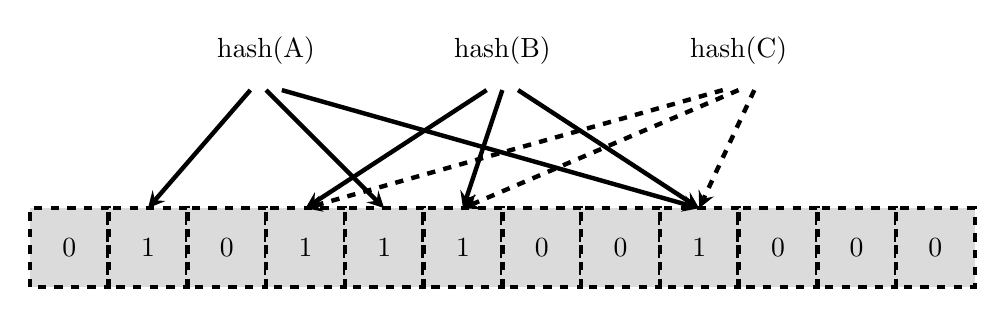
\begin{tikzpicture}

 \draw[ultra thick, fill=black!14, dashed] (0, 0) rectangle (1, 1);
 \draw[ultra thick, fill=black!14, dashed] (1, 0) rectangle (2, 1);
 \draw[ultra thick, fill=black!14, dashed] (2, 0) rectangle (3, 1);
 \draw[ultra thick, fill=black!14, dashed] (3, 0) rectangle (4, 1);
 \draw[ultra thick, fill=black!14, dashed] (4, 0) rectangle (5, 1);
 \draw[ultra thick, fill=black!14, dashed] (5, 0) rectangle (6, 1);
 \draw[ultra thick, fill=black!14, dashed] (6, 0) rectangle (7, 1);
 \draw[ultra thick, fill=black!14, dashed] (7, 0) rectangle (8, 1);
 \draw[ultra thick, fill=black!14, dashed] (8, 0) rectangle (9, 1);
 \draw[ultra thick, fill=black!14, dashed] (9, 0) rectangle (10, 1);
 \draw[ultra thick, fill=black!14, dashed] (10, 0) rectangle (11, 1);
 \draw[ultra thick, fill=black!14, dashed] (11, 0) rectangle (12, 1);
 \node at (0.5, 0.5) {0};
 \node at (1.5, 0.5) {1};
 \node at (2.5, 0.5) {0};
 \node at (3.5, 0.5) {1};
 \node at (4.5, 0.5) {1};
 \node at (5.5, 0.5) {1};
 \node at (6.5, 0.5) {0};
 \node at (7.5, 0.5) {0};
 \node at (8.5, 0.5) {1};
 \node at (9.5, 0.5) {0};
 \node at (10.5, 0.5) {0};
 \node at (11.5, 0.5) {0};

 \node at(3, 3) {hash(A)};
 \node at(6, 3) {hash(B)};
 \node at(9, 3) {hash(C)};

 \draw[-stealth, ultra thick] (2.8, 2.5) to (1.5, 1);
 \draw[-stealth, ultra thick] (3, 2.5) to (4.5, 1);
 \draw[-stealth, ultra thick] (3.2, 2.5) to (8.5, 1);

 \draw[-stealth, ultra thick] (5.8, 2.5) to (3.5, 1);
 \draw[-stealth, ultra thick] (6, 2.5) to (5.5, 1);
 \draw[-stealth, ultra thick] (6.2, 2.5) to (8.5, 1);

 \draw[-stealth, ultra thick, dashed] (8.8, 2.5) to (3.5, 1);
 \draw[-stealth, ultra thick, dashed] (9, 2.5) to (5.5, 1);
 \draw[-stealth, ultra thick, dashed] (9.2, 2.5) to (8.5, 1);
 
 \end{tikzpicture}

  \caption{How a false positive (``C'') can arise in toy Bloom filter. ``C'' is hashed to 3 different positions. However, it found that all the three positions are $1$. So the Bloom filter fails to classify the fingerprint ``C'' as unique.}
  \label{fig:bloom-filter}
\end{figure}

\fi


\subsection{Fingerprint management}

Lazy deduplication aims at decreasing disk access time by deferring and merging on-disk fingerprint lookups.  Fingerprints which need to be looked up on disk are initially stored in an in-memory hash table, the \emph{buffer}.  They are stored until the number of fingerprints in a hash bucket reaches a threshold, which we refer to as the \emph{buffer fingerprint threshold} (BFT).  When the threshold is reached, all of the fingerprints within the hash bucket are searched for on disk.  Figure~\ref{fig:lazy-method} illustrates the underlying idea behind lazy method.  The system searches for the in-buffer bucket fingerprints among the on-disk buckets with the same bucket ID using a fingerprint-to-bucket function, proceeding bucket by bucket.  Fingerprints not found are unique, which are ``false positives'' by the Bloom filter.


Fingerprints are stored on disk in two ways:
\begin{itemize}
 \item Unique fingerprints are stored in an \emph{on-disk hash table}, which is used to facilitate searching.  The on-disk hash table and the buffer use the same hash function.  For the on-disk hash table, we use separate chaining to resolve bucket overflow.
 \item Both unique and duplicate fingerprints are stored in a log-structured \emph{metadata} array.  They are stored in the order in which they arrive, thereby preserving locality. A fingerprint in the on-disk hash table points to the corresponding metadata entry, and the neighboring metadata entries are prefetched into the cache when one fingerprint is found in the on-disk hash table.
\end{itemize}

This method could easily be adapted for systems like ChunkStash~\cite{debnath2010chunkstash} or BloomStore~\cite{lu2012bloomstore}, as they also use a hash table to organize fingerprints. Specifically, we could similarly perform on-disk searching in batches within search spaces restricted by hash values.


\begin{figure}[htbp]
  \begin{center}
  \includegraphics[width=0.6\columnwidth]{idea}
  \end{center}
  \caption{Illustration of the lazy method.  Three fingerprints are buffered in hash bucket $1$, making it full. Together, they are searched for on disk among the fingerprints with the same bucket ID using a fingerprint-to-bucket function.  Here, we use ``fp'' to denote an arbitrary fingerprint, and $n$ to denote the length of the hash index.}
  \label{fig:lazy-method}
\end{figure}

To buffer the fingerprints, the lazy method requires additional memory space, and since we cannot know \textit{a priori} which chunks are duplicates, the data chunks need to be buffered too. Assume a hash table with $n$ buckets is used to buffer the fingerprints, the size of each fingerprint is $S_\text{fp}$, BFT is set to $T$, and the average chunk size is $S_\text{chk}$. Then the memory required to buffer the fingerprints is $$\text{Space}_\text{fp}:=n S_\text{fp}T$$ and the average memory occupied by the corresponding chunks is $$\text{Space}_\text{chk}:=n S_\text{chk}T.$$ So the extra space required is given by 
\begin{align*}
\mathrm{Space} &:=\mathrm{Space}_\text{fp}+\mathrm{Space}_\text{chk} \\
 &=(S_\text{fp}+S_\text{chk})n T.
\end{align*}

If e.g.,\ SHA1 is the fingerprint algorithm and we set the average chunk size to $4$KB, which are typical in deduplication systems, the number of hash buckets $n=1024$, and BFT is set to $32$, then $\mathrm{Space} \simeq 128$MB, acceptable cost on modern hardware.


An entry in an on-disk hash bucket will have size around $40$B, comprising of the fingerprint itself, a pointer to the corresponding metadata entry and some other information. (The entry size will depend on the choice of cryptographic hash function and the size of the pointers.)  A $4$MB hash bucket can therefore contain around $100{,}000$ entries, and, assuming there's a single $4$MB hash bucket in each hash index slot, the whole on-disk hash table can support $1024 \times 100,000 \times 4\text{KB} \simeq 400$GBs of unique data.  With a BFT set to $32$, the buffer will have at most $32 \times 1024$ fingerprints in it at a given time, for which we need to reserve at least $32 \times 1024 \times 4\text{KB}=128$MBs of memory for storing the corresponding chunks. This guarantees the system identifies $32$ fingerprints per disk I/O.

By adjusting the number of hash buckets $n$, the amount of unique data supported by the on-disk hash table scales linearly with the amount of memory we need to reserve for the buffer.  Thus, $m$GBs of memory allocated to the buffer is required for a data set with $\simeq 3000m$GBs of unique data.  Duplicate fingerprints will not appear in the on-disk hash table.

Should this be a limiting factor, we can either adjust the hash bucket size or use a chain-based on-disk hash table (illustrated Figure~\ref{fig:lazy-method}), where each hash slot indexes multiple buckets.  However, both of these would reduce the search performance.


\subsection{Caching Strategy}

Fingerprint caching has proven to be a significant factor in data deduplication systems. Repeated patterns in backup data streams have been leveraged to design effective cache strategies to minimize disk accesses~\cite{bhagwat2009extreme,guo2011building,lillibridge2009sparse,manber1994finding,xia2011silo,zhu2008avoiding}.

For the eager method, Figure~\ref{fig:cache-eager} illustrates how locality is exploited in caching.  Data chunks often arrive in a similar order to which they came previously, so when a fingerprint is found on disk, the subsequent on-disk fingerprints are prefetched into the cache. When subsequent incoming fingerprints arrive, they are often found among these prefetched fingerprints, resulting in cache hits.

\begin{figure}[htbp]
\centering

\subfloat[The first encounter.  The fingerprints are written to disk in the order in which they arrive so that locality is preserved.]{
\resizebox{0.45\textwidth}{!}{
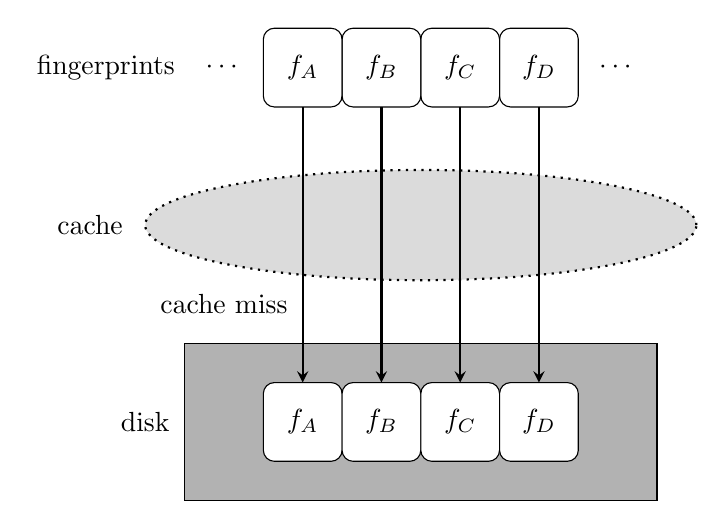
\begin{tikzpicture}
 \node at (1,0.5) {fingerprints};
 \node at (0.8,-1.5) {cache};
 \node at (1.5,-4) {disk};
 \node at (2.5,-2.5) {cache miss};

 \draw[rounded corners] (3,0) rectangle (4,1);
 \draw[rounded corners] (4,0) rectangle (5,1);
 \draw[rounded corners] (5,0) rectangle (6,1);
 \draw[rounded corners] (6,0) rectangle (7,1);
 \node at (2.5,0.5) {$\cdots$};
 \node at (3.5,0.5) {$f_A$};
 \node at (4.5,0.5) {$f_B$};
 \node at (5.5,0.5) {$f_C$};
 \node at (6.5,0.5) {$f_D$};
 \node at (7.5,0.5) {$\cdots$};

 \draw[fill=black!30] (2,-3) rectangle (8,-5);
 
 \draw[thick,fill=black!14,dotted] (5,-1.5) ellipse (3.5 and 0.7);
 \draw[thick,-stealth] (3.5,0) -> (3.5,-3.5);
 \draw[thick,-stealth] (4.5,0) -> (4.5,-3.5);
 \draw[thick,-stealth] (5.5,0) -> (5.5,-3.5);
 \draw[thick,-stealth] (6.5,0) -> (6.5,-3.5);
 
 \draw[fill=white,rounded corners] (3,-4.5) rectangle (4,-3.5);
 \draw[fill=white,rounded corners] (4,-4.5) rectangle (5,-3.5);
 \draw[fill=white,rounded corners] (5,-4.5) rectangle (6,-3.5);
 \draw[fill=white,rounded corners] (6,-4.5) rectangle (7,-3.5);
 \node at (3.5,-4) {$f_A$};
 \node at (4.5,-4) {$f_B$};
 \node at (5.5,-4) {$f_C$};
 \node at (6.5,-4) {$f_D$};
\end{tikzpicture}
}
}
\quad
\subfloat[A subsequent encounter.  The fingerprint $f_A$ is found on disk, and subsequent fingerprints are prefetched.]{
\centering
\resizebox{0.45\textwidth}{!}{
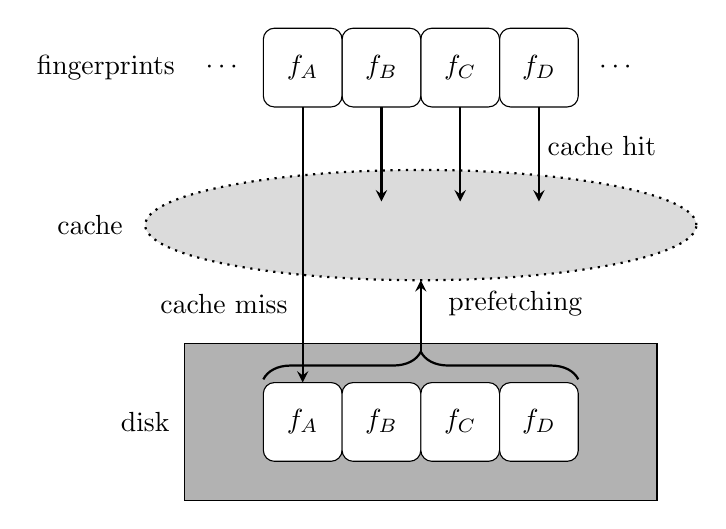
\begin{tikzpicture}
 \node at (1,0.5) {fingerprints};
 \node at (0.8,-1.5) {cache};
 \node at (2.5,-2.5) {cache miss};
 \node at (6.2,-2.5) {prefetching};
 \node at (1.5,-4) {disk};
 \node at (7.3,-0.5) {cache hit};

 \draw[rounded corners] (3,0) rectangle (4,1);
 \draw[rounded corners] (4,0) rectangle (5,1);
 \draw[rounded corners] (5,0) rectangle (6,1);
 \draw[rounded corners] (6,0) rectangle (7,1);
 \node at (2.5,0.5) {$\cdots$};
 \node at (3.5,0.5) {$f_A$};
 \node at (4.5,0.5) {$f_B$};
 \node at (5.5,0.5) {$f_C$};
 \node at (6.5,0.5) {$f_D$};
 \node at (7.5,0.5) {$\cdots$};

 \draw[fill=black!30] (2,-3) rectangle (8,-5);
 
 \draw[thick,fill=black!14,dotted] (5,-1.5) ellipse (3.5 and 0.7);
 \draw[thick,-stealth] (3.5,0) -> (3.5,-3.5);
 
 \draw[thick,-stealth] (4.5,0) -> (4.5,-1.2);
 \draw[thick,-stealth] (5.5,0) -> (5.5,-1.2);
 \draw[thick,-stealth] (6.5,0) -> (6.5,-1.2);
 
 \draw[fill=white,rounded corners] (3,-4.5) rectangle (4,-3.5);
 \draw[fill=white,rounded corners] (4,-4.5) rectangle (5,-3.5);
 \draw[fill=white,rounded corners] (5,-4.5) rectangle (6,-3.5);
 \draw[fill=white,rounded corners] (6,-4.5) rectangle (7,-3.5);
 \node at (3.5,-4) {$f_A$};
 \node at (4.5,-4) {$f_B$};
 \node at (5.5,-4) {$f_C$};
 \node at (6.5,-4) {$f_D$};
 
 \draw [thick,decorate,decoration={brace,amplitude=10pt,mirror,raise=4pt},yshift=0pt] (7,-3.6) -- (3,-3.6);
 \draw[thick,stealth-] (5,-2.2) -> (5,-3.1);
\end{tikzpicture}
}
}

\caption{Illustrating caching in the eager method and how data locality is exploited.  The fingerprints $f_A$, $f_B$, $f_C$, and $f_D$ are processed in order, and are stored on disk in that order to facilitate later prefetching.}
\label{fig:cache-eager}
\end{figure}

In the lazy method, fingerprints will instead be buffered, so we cannot use the same caching strategy as eager deduplication.  Figure~\ref{fig:cache-lazy} modifies Figure~\ref{fig:cache-eager} showing the caching method used in lazy deduplication.  Fingerprints are buffered when processing the data stream, and will not be looked up on disk until their corresponding hash bucket is full. Subsequent incoming fingerprints will arrive before prefetching occurs, and will therefore be buffered too.

This caching strategy introduces two issues: (a) we need to decide which fingerprints should be prefetched, and (b) we need to decide which fingerprints in the buffer should be searched for in the cache after prefetching.  These are addressed by using ``buffer cycles'' and recording a ``rank''.


\begin{figure}[htbp]
\centering
\resizebox{0.6\columnwidth}{!}{
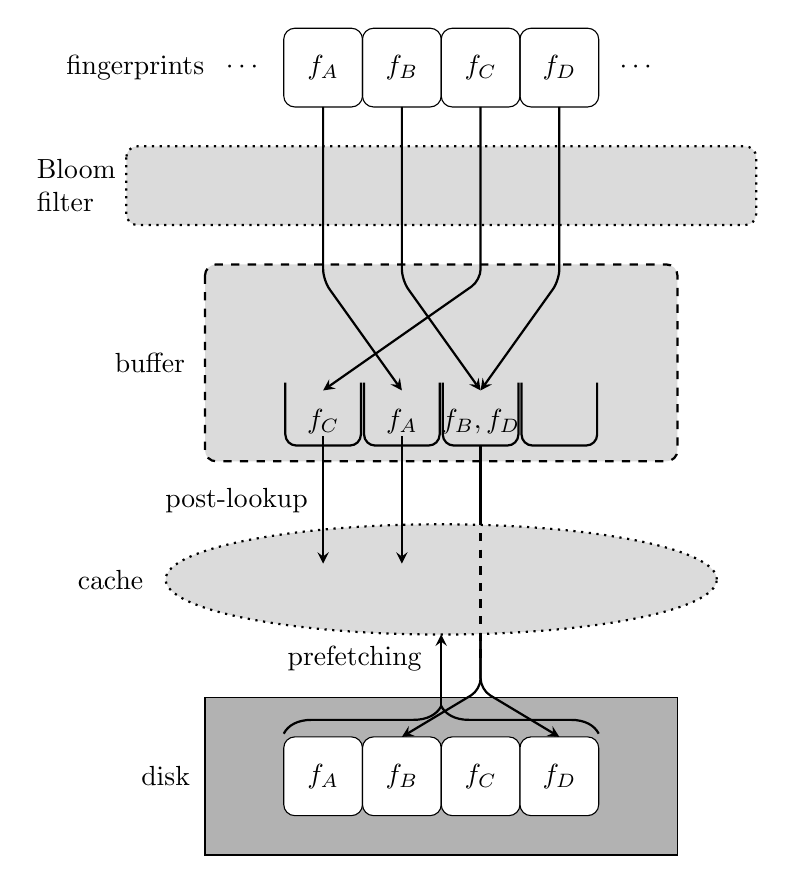
\begin{tikzpicture}
 \node at (1,0.5) {\parbox{0.6in}{fingerprints}};
 \node at (0.5,-1) {\parbox{0.5in}{Bloom filter}};
 \node at (0.8,-6) {cache};
 \node at (2.4,-5) {post-lookup};
% \node at (6.4,-7) {cache miss};
 \node at (3.9,-7) {prefetching};
 \node at (1.5,-8.5) {disk};
 \node at (1.3,-3.25) {buffer};

 \draw[rounded corners] (3,0) rectangle (4,1);
 \draw[rounded corners] (4,0) rectangle (5,1);
 \draw[rounded corners] (5,0) rectangle (6,1);
 \draw[rounded corners] (6,0) rectangle (7,1);
 \node at (2.5,0.5) {$\cdots$};
 \node at (3.5,0.5) {$f_A$};
 \node at (4.5,0.5) {$f_B$};
 \node at (5.5,0.5) {$f_C$};
 \node at (6.5,0.5) {$f_D$};
 \node at (7.5,0.5) {$\cdots$};
 \draw[thick,fill=black!14,dotted,rounded corners] (1,-0.5) rectangle (9,-1.5);
 \draw[thick,fill=black!14,dashed,rounded corners] (2,-2) rectangle (8,-4.5);
 
 \draw[thick,-stealth,rounded corners] (3.5,0) -- (3.5,-2.2) -- (4.5,-3.6);
 \draw[thick,-stealth,rounded corners] (4.5,0) -- (4.5,-2.2) -- (5.5,-3.6);
 \draw[thick,-stealth,rounded corners] (5.5,0) -- (5.5,-2.2) -- (3.5,-3.6);
 \draw[thick,-stealth,rounded corners] (6.5,0) -- (6.5,-2.2) -- (5.5,-3.6);
 
 \draw[thick,rounded corners] (3.02,-3.5) -- (3.02,-4.3) -- (3.98,-4.3) -- (3.98,-3.5);
 \draw[thick,rounded corners] (4.02,-3.5) -- (4.02,-4.3) -- (4.98,-4.3) -- (4.98,-3.5);
 \draw[thick,rounded corners] (5.02,-3.5) -- (5.02,-4.3) -- (5.98,-4.3) -- (5.98,-3.5);
 \draw[thick,rounded corners] (6.02,-3.5) -- (6.02,-4.3) -- (6.98,-4.3) -- (6.98,-3.5);
 
 \node at (3.5,-4) {$f_C$};
 \node at (4.5,-4) {$f_A$};
 \node at (5.5,-4) {$f_B,f_D$};
 \node at (6.5,-4) {};
 
 \draw[thick,fill=black!14,dotted] (5,-6) ellipse (3.5 and 0.7);
 \draw[fill=black!30] (2,-7.5) rectangle (8,-9.5);

 
 \draw[fill=white,rounded corners] (3,-8) rectangle (4,-9);
 \draw[fill=white,rounded corners] (4,-8) rectangle (5,-9);
 \draw[fill=white,rounded corners] (5,-8) rectangle (6,-9);
 \draw[fill=white,rounded corners] (6,-8) rectangle (7,-9);
 \node at (3.5,-8.5) {$f_A$};
 \node at (4.5,-8.5) {$f_B$};
 \node at (5.5,-8.5) {$f_C$};
 \node at (6.5,-8.5) {$f_D$};
 
 \draw[thick,rounded corners] (5.5,-4.3) -- (5.5,-5.2);
 \draw[thick,dashed,rounded corners] (5.5,-5.2) -- (5.5,-7);
 
 \draw[thick,-stealth,rounded corners] (5.5,-6.7) -- (5.5,-7.4) -- (4.5,-8);
 \draw[thick,-stealth,rounded corners] (5.5,-6.7) -- (5.5,-7.4) -- (6.5,-8);
 
 \draw [thick,decorate,decoration={brace,amplitude=10pt,mirror,raise=4pt},yshift=0pt] (7,-8.1) -- (3,-8.1);
 \draw[thick,stealth-] (5,-6.7) -> (5,-7.62);
 
 \draw[thick,-stealth] (3.5,-4.18) -> (3.5,-5.8);
 \draw[thick,-stealth] (4.5,-4.18) -> (4.5,-5.8);
\end{tikzpicture}
}
\caption{Illustrating caching in the lazy method.  The fingerprints $f_A$, $f_B$, $f_C$, and $f_D$ are buffered, and when one of the hash buckets is full, it is looked up on disk as a batch (without checking the cache).  This triggers prefetching, after which post-lookup is performed and, as a result, fingerprints $f_A$ and $f_C$ are found in the cache.}
\label{fig:cache-lazy}
\end{figure}

In addition to the hash table, fingerprints that reach the buffer are inserted into a \emph{buffer cycle}, a cyclic data structure where pointers indicate the previous and next fingerprints in the cycle.   They are also stored with a number $r$, which we call the \emph{rank}, which gives the order in which fingerprints arrive.  The first fingerprint in a cycle has rank $0$ and the subsequent fingerprints have rank $1,2,\ldots$, including both unique and duplicate fingerprints.  This is illustrated in Figure~\ref{fig:list-buffer}. Algorithm~\ref{alg:circle} gives the procedure how to construct the buffer cycle.

% Algorithm
\begin{algorithm}[htbp]
\SetAlgoNoLine
\KwIn{fingerprints $f_1, f_2,\ldots$.}
%\KwOut{The frequency number ($FreNum_{\alpha}$) node $\alpha$ gets assigned.}
% mjw: The unique length is used to separate unrelated sequence. MAX_CIRCLE_LENGTH and MAX_RANK is the same
$\mathrm{MAX\_UNIQUE\_LENGTH}$=200; $\mathrm{MAX\_CYCLE\_LENGTH}$=2048; $\mathrm{Uniques} \gets 0$; $\mathrm{Rank} \gets 0$\;
\For{each fingerprint $f_i$}{
    Test $f_i$ using Bloom filter\;
    \eIf{$f_i$ is found to be unique}
    {
    $\mathrm{Uniques} \gets \mathrm{Uniques} + 1$\;
    \If{$\mathrm{Uniques} > \mathrm{MAX\_UNIQUE\_LENGTH}$}{$\mathrm{Rank} \gets 0$\; $\mathrm{Uniques} \gets 0$\; Start a new buffer cycle;}
    }
    {
    $\mathrm{Rank} \gets \mathrm{Rank} + \mathrm{Uniques}$\; $\mathrm{Uniques} \gets 0$\;
    Pre-lookup $f_i$ in the cache\;
    \If{$f_i$ is not found in the cache}
    {
    \If{$\mathrm{Rank} > \mathrm{MAX\_CYCLE\_LENGTH}$}{$\mathrm{Rank} \gets 0$\; Start a new buffer cycle;}
    assign $\mathrm{Rank}$ to $f_i$ and append it to the current list
    }
    $\mathrm{Rank} \gets \mathrm{Rank} + 1$\;
    }
}
\caption{Construction of the buffer cycles.}
\label{alg:circle}
\end{algorithm}


\begin{figure}[htbp]
  \begin{center}
  \includegraphics[width=0.6\columnwidth]{list-buffer}
  \end{center}
  \caption{An example of a buffer cycle and the fingerprint ranks $r$.  In this example, a new buffer cycle is created when the fingerprint $f_A$ arrives, which begins a sequence of $26$ consecutive fingerprints $f_A,f_B,\ldots,f_Z$, of which all except $f_C$ (not shown) are buffered.  No fingerprint in this buffer cycle has rank $2$.}
  \label{fig:list-buffer}
\end{figure}

Buffer cycles and the rank are used to facilitate bidirectional prefetching: when a fingerprint with rank $r$ is searched for on disk, we prefetch a sequence of $N$ consecutive fingerprints (we use $N=2048$), starting from the $r$-th preceeding fingerprint.  The fingerprints in the buffer cycle are likely to have matching, prefetched fingerprints. So the system searches the fingerprints in the same cycle after prefetching.  Figure~\ref{fig:cycle_rank} illustrates the roles of a buffer cycle and ranks.

\begin{figure}[htbp]
\centering
\resizebox{\textwidth}{!}{
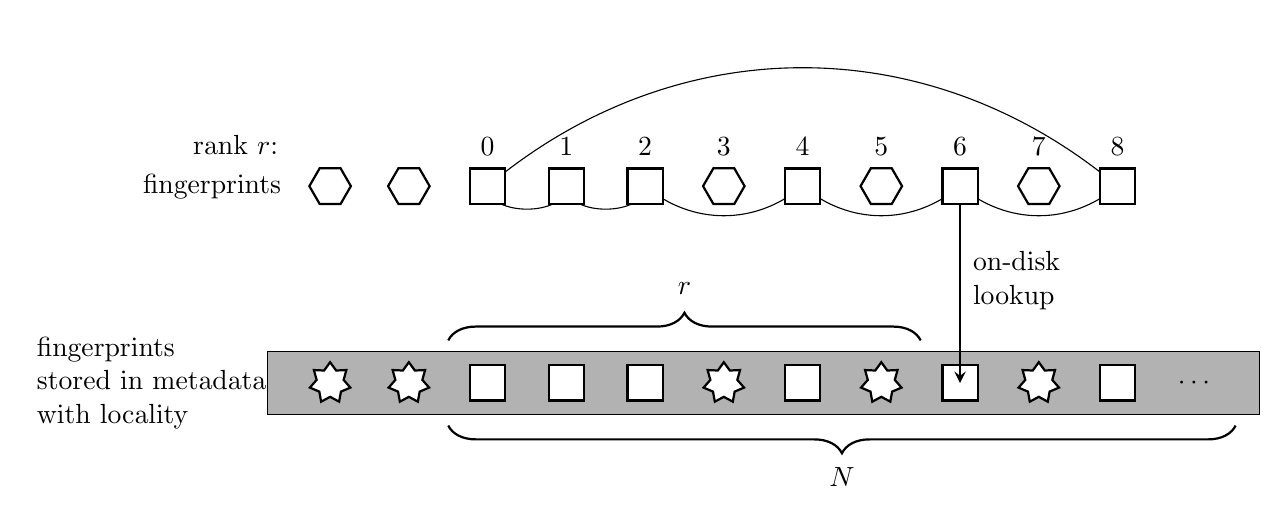
\begin{tikzpicture}
 \draw (6,0) to[bend right=40] (8,0);
 \draw (8,0) to[bend right=40] (10,0);
 \draw (2,0) to[bend left=40] (10,0);
 \draw (2,0) to[bend right=90] (3,0);
 \draw (3,0) to[bend right=90] (4,0);
 \draw (4,0) to[bend right=40] (6,0);
 
 \node[thick,regular polygon,regular polygon sides=6,draw,inner sep=0pt,minimum width=15pt,fill=white] at (0,0) {};
 \node[thick,regular polygon,regular polygon sides=6,draw,inner sep=0pt,minimum width=15pt,fill=white] at (1,0) {};
 \node[thick,regular polygon,regular polygon sides=4,draw,inner sep=0pt,minimum width=18pt,fill=white] at (2,0) {};
 \node[thick,regular polygon,regular polygon sides=4,draw,inner sep=0pt,minimum width=18pt,fill=white] at (3,0) {};
 \node[thick,regular polygon,regular polygon sides=4,draw,inner sep=0pt,minimum width=18pt,fill=white] at (4,0) {};
 \node[thick,regular polygon,regular polygon sides=6,draw,inner sep=0pt,minimum width=15pt,fill=white] at (5,0) {};
 \node[thick,regular polygon,regular polygon sides=4,draw,inner sep=0pt,minimum width=18pt,fill=white] at (6,0) {};
 \node[thick,regular polygon,regular polygon sides=6,draw,inner sep=0pt,minimum width=15pt,fill=white] at (7,0) {};
 \node[thick,regular polygon,regular polygon sides=4,draw,inner sep=0pt,minimum width=18pt,fill=white] at (8,0) {};
 \node[thick,regular polygon,regular polygon sides=6,draw,inner sep=0pt,minimum width=15pt,fill=white] at (9,0) {};
 \node[thick,regular polygon,regular polygon sides=4,draw,inner sep=0pt,minimum width=18pt,fill=white] at (10,0) {};
 
 \node at (-1.2,0.53) {rank $r$:};
 \node at (-1.5,0) {fingerprints};
 
 \node at (2,0.5) {$0$};
 \node at (3,0.5) {$1$};
 \node at (4,0.5) {$2$};
 \node at (5,0.5) {$3$};
 \node at (6,0.5) {$4$};
 \node at (7,0.5) {$5$};
 \node at (8,0.5) {$6$};
 \node at (9,0.5) {$7$};
 \node at (10,0.5) {$8$};
 
 \node at (-2.2,-2.5) {\parbox{1.2in}{fingerprints \\ stored in metadata \\ with locality}};
 \node at (8.8,-1.2) {\parbox{0.5in}{on-disk \\ lookup}};
 \draw[fill=black!30] (-0.8,-2.1) rectangle (11.8,-2.9);

 \node[thick,star,star points=7,draw,inner sep=0pt,minimum width=15pt,fill=white] at (0,-2.5) {};
 \node[thick,star,star points=7,draw,inner sep=0pt,minimum width=15pt,fill=white] at (1,-2.5) {};
 \node[thick,regular polygon,regular polygon sides=4,draw,inner sep=0pt,minimum width=18pt,fill=white] at (2,-2.5) {};
 \node[thick,regular polygon,regular polygon sides=4,draw,inner sep=0pt,minimum width=18pt,fill=white] at (3,-2.5) {};
 \node[thick,regular polygon,regular polygon sides=4,draw,inner sep=0pt,minimum width=18pt,fill=white] at (4,-2.5) {};
 \node[thick,star,star points=7,draw,inner sep=0pt,minimum width=15pt,fill=white] at (5,-2.5) {};
 \node[thick,regular polygon,regular polygon sides=4,draw,inner sep=0pt,minimum width=18pt,fill=white] at (6,-2.5) {};
 \node[thick,star,star points=7,draw,inner sep=0pt,minimum width=15pt,fill=white] at (7,-2.5) {};
 \node[thick,regular polygon,regular polygon sides=4,draw,inner sep=0pt,minimum width=18pt,fill=white] at (8,-2.5) {};
 \node[thick,star,star points=7,draw,inner sep=0pt,minimum width=15pt,fill=white] at (9,-2.5) {};
 \node[thick,regular polygon,regular polygon sides=4,draw,inner sep=0pt,minimum width=18pt,fill=white] at (10,-2.5) {};
 \node[] at (11,-2.5) {$\cdots$};

 \draw[thick,-stealth] (8,-0.22) to (8,-2.5);

 \draw [thick,decorate,decoration={brace,amplitude=10pt,mirror,raise=4pt},yshift=0pt] (1.5,-2.9) -- (11.5,-2.9) node [black,midway,yshift=-0.8cm] {$N$};
 \draw [thick,decorate,decoration={brace,amplitude=10pt,mirror,raise=4pt},yshift=0pt] (7.5,-2.1) -- (1.5,-2.1) node [black,midway,yshift=0.8cm] {$r$};
\end{tikzpicture}
}
\caption{Illustrating the role of a buffer cycle and the rank in prefetching. Squares represent duplicate candidates, while hexagon and stars represent unique (and therefore distinct) fingerprints in two sequences. The incoming fingerprints drawn as squares are those that are buffered (i.e., they pass through the Bloom filter and are not found during pre-lookup); one by one, they are inserted into the current buffer cycle.  An on-disk lookup is performed for some fingerprint, and we prefetch $N$ surrounding on-disk fingerprints starting from the $r$-th preceding fingerprint.  If a similar sequence of fingerprints has occurred previously, it will be prefetched into the cache, and the buffer cycle tells us which fingerprints to look for in the cache.}
\label{fig:cycle_rank}
\end{figure}

When a fingerprint passes through the Bloom filter it is usually a duplicate, and if it's not found during pre-lookup we insert it into the current buffer cycle.  Some (necessarily unique) fingerprints will be filtered out by the Bloom filter, while appearing within sequences of duplicate fingerprints.  This situation often arises as the result of small modifications to a file.  Fingerprints which don't make it to the buffer are not added to a buffer cycle, but we keep track of their existence using the rank.

If the number of consecutive fingerprints filtered out by the Bloom filter exceeds a threshold (we use $200$), we start a new cycle starting with the next duplicate fingerprint.  When the length of the cycle reaches the maximum allowed length (chosen to equal the prefetching volume, so all the fingerprints in the same cycle are expected to be covered by the prefetching), we also start a new cycle and add the incoming duplicate fingerprint to the new cycle.

There will generally be many buffer cycles (one of which being the ``current'' buffer cycle, to which fingerprints are added), and every fingerprint in the buffer will ordinarily belong to a unique buffer cycle. When a hash bucket becomes full, the fingerprints in it will be searched for on the disk. Fingerprints not found on the disk are unique and are written to disk. Fingerprints found on the disk are duplicates, and when found, prefetching is triggered. After prefetching, the fingerprints in the same cycle are searched for in the cache (i.e., post-lookup). We use the Least Recently Used (LRU) eviction strategy to update the cache; newly added fingerprints stay longer to facilitate the flowing pre-lookups.

Some fingerprints will be searched for in the cache several times.  This happens for unique fingerprints (which pass through the Bloom filter), and for fingerprints without locality with the fingerprints in the same buffer cycle. To alleviate this, we limit the number of cache lookups per fingerprint in the buffer to $10$, after which the system removes the fingerprint from its buffer cycle. For fingerprints outside of buffer cycles, prefetching is not triggered after it is found on disk, avoiding disk I/O for prefetching for fingerprints without locality.


\subsection{Computing optimization on a multi-core platform}

As the proportion of deduplication time spent on disk accesses decreases, the proportion of time spent on computational tasks becomes the new bottleneck (although even in the eager method, these tasks are not entirely negligible).  Thus, we also aim to reduce the time spent on these computational tasks.

With Moore's Law ``coming to an end'' \cite{Waldrop2016}, CPU frequency is developing comparatively slowly, being replaced by increases in the number of CPU cores.  Additionally, GPUs are increasingly being utilized in scientific computing, some of which have thousands of cores, providing powerful parallel computing resources.  However, software needs to be redesigned to meaningfully utilize the GPU's highly parallel hardware.  Parallel hardware allows us to overlap computational tasks (in the case of multi-core hardware) or offload them to reduce the CPU load (in the case of the GPU).

Figure~\ref{fig:thread} illustrates how the CPU and GPU threads process the data chunks in our deduplication implementation.  The granularity on the CPU and GPU differ. On the GPU, we assign an individual thread to processing an individual chunk, while a CPU thread processes a batch of data.  The many-core GPU hardware makes it better utilized when assigned many similar-sized tasks.  However, in deduplication, this requires transfers from the main memory to the GPU memory; we reduce the number of transfers by batching.  In the CPU side, assigning a batch of chunks to a CPU thread avoids problems arising from frequent thread switches.

\begin{figure}[htbp]
\centering
% \resizebox{0.8\columnwidth}{!}{
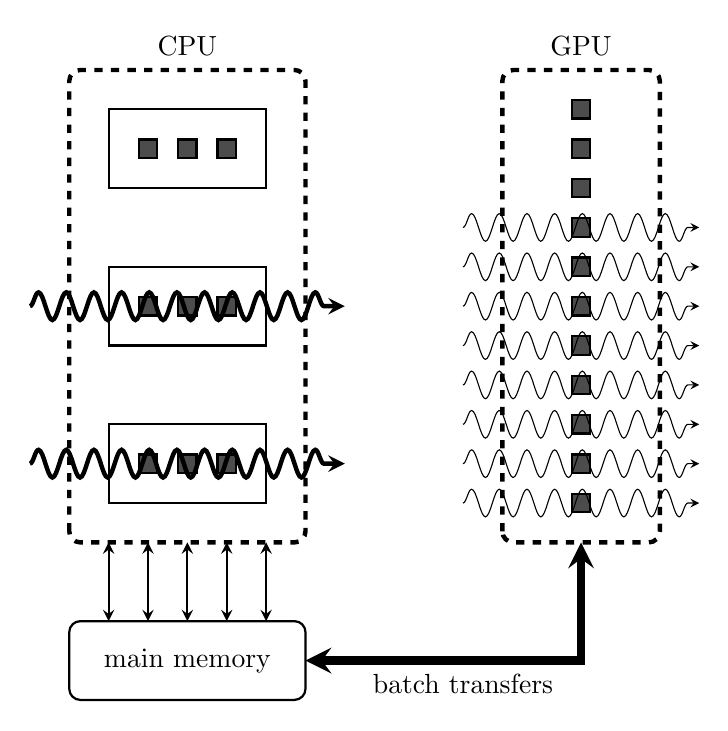
\begin{tikzpicture}
 \draw[ultra thick,dashed,rounded corners] (0.5,0.5) rectangle (3.5,6.5);
 
 \draw[thick,fill=white] (1,1) rectangle (3,2);
 \node[draw,thick,fill=black!70] at (1.5,1.5) {};
 \node[draw,thick,fill=black!70] at (2,1.5) {};
 \node[draw,thick,fill=black!70] at (2.5,1.5) {};

 \draw[thick,fill=white] (1,3) rectangle (3,4);
 \node[draw,thick,fill=black!70] at (1.5,3.5) {};
 \node[draw,thick,fill=black!70] at (2,3.5) {};
 \node[draw,thick,fill=black!70] at (2.5,3.5) {};
 
 \draw[thick,fill=white] (1,5) rectangle (3,6);
 \node[draw,thick,fill=black!70] at (1.5,5.5) {};
 \node[draw,thick,fill=black!70] at (2,5.5) {};
 \node[draw,thick,fill=black!70] at (2.5,5.5) {};
 
 \draw[ultra thick,-stealth, decorate, decoration={snake,amplitude=5pt,post length=3pt}] (0,1.5) -- (4,1.5);
 \draw[ultra thick,-stealth, decorate, decoration={snake,amplitude=5pt,post length=3pt}] (0,3.5) -- (4,3.5);
 
 \draw[ultra thick,dashed,rounded corners] (6,0.5) rectangle (8,6.5);
 
 \node[draw,thick,fill=black!70] at (7,1) {};
 \node[draw,thick,fill=black!70] at (7,1.5) {};
 \node[draw,thick,fill=black!70] at (7,2) {};
 \node[draw,thick,fill=black!70] at (7,2.5) {};
 \node[draw,thick,fill=black!70] at (7,3) {};
 \node[draw,thick,fill=black!70] at (7,3.5) {};
 \node[draw,thick,fill=black!70] at (7,4) {};
 \node[draw,thick,fill=black!70] at (7,4.5) {};
 \node[draw,thick,fill=black!70] at (7,5) {};
 \node[draw,thick,fill=black!70] at (7,5.5) {};
 \node[draw,thick,fill=black!70] at (7,6) {};
 
 \draw[thin,-stealth, decorate, decoration={snake,amplitude=5pt,post length=3pt}] (5.5,1) -- (8.5,1);
 \draw[thin,-stealth, decorate, decoration={snake,amplitude=5pt,post length=3pt}] (5.5,1.5) -- (8.5,1.5);
 \draw[thin,-stealth, decorate, decoration={snake,amplitude=5pt,post length=3pt}] (5.5,2) -- (8.5,2);
 \draw[thin,-stealth, decorate, decoration={snake,amplitude=5pt,post length=3pt}] (5.5,2.5) -- (8.5,2.5);
 \draw[thin,-stealth, decorate, decoration={snake,amplitude=5pt,post length=3pt}] (5.5,3) -- (8.5,3);
 \draw[thin,-stealth, decorate, decoration={snake,amplitude=5pt,post length=3pt}] (5.5,3.5) -- (8.5,3.5);
 \draw[thin,-stealth, decorate, decoration={snake,amplitude=5pt,post length=3pt}] (5.5,4) -- (8.5,4);
 \draw[thin,-stealth, decorate, decoration={snake,amplitude=5pt,post length=3pt}] (5.5,4.5) -- (8.5,4.5);
 
 \draw[thick,rounded corners] (0.5,-0.5) rectangle (3.5,-1.5);
 \node at (2,-1) {main memory};
 
 \node at (2,6.8) {CPU};
 \node at (7,6.8) {GPU};
 
 \draw[line width=3pt,stealth-stealth] (3.5,-1) -| (7,0.5);
 
 \draw[thick,stealth-stealth] (1,-0.5) -- (1,0.5);
 \draw[thick,stealth-stealth] (1.5,-0.5) -- (1.5,0.5);
 \draw[thick,stealth-stealth] (2,-0.5) -- (2,0.5);
 \draw[thick,stealth-stealth] (2.5,-0.5) -- (2.5,0.5);
 \draw[thick,stealth-stealth] (3,-0.5) -- (3,0.5);
 
 \node at (5.5,-1.3) {batch transfers};
 
\end{tikzpicture}
% }

\caption{Illustrating parallel processing of processing chunks on the CPU and GPU.  On the CPU side, CPU threads process chunks as batches, and repeated main memory access is not a major concern.  On the GPU side, individual threads are assigned individual chunks to process, and we reduce the number of main memory accesses by using batching.}
\label{fig:thread}
\end{figure}

Figure~\ref{fig:gpu-data} illustrates the data transfer procedure. In our prototype, we use the GPU to accelerate the SHA1 calculation.  The host transfers a batch of chunks to the GPU memory, after which the GPU computes the SHA1-value of each chunk. The host then transfers the calculated fingerprints from the GPU memory to the main memory.

\begin{figure}[htbp]
\centering
%\resizebox{\textwidth}{!}{
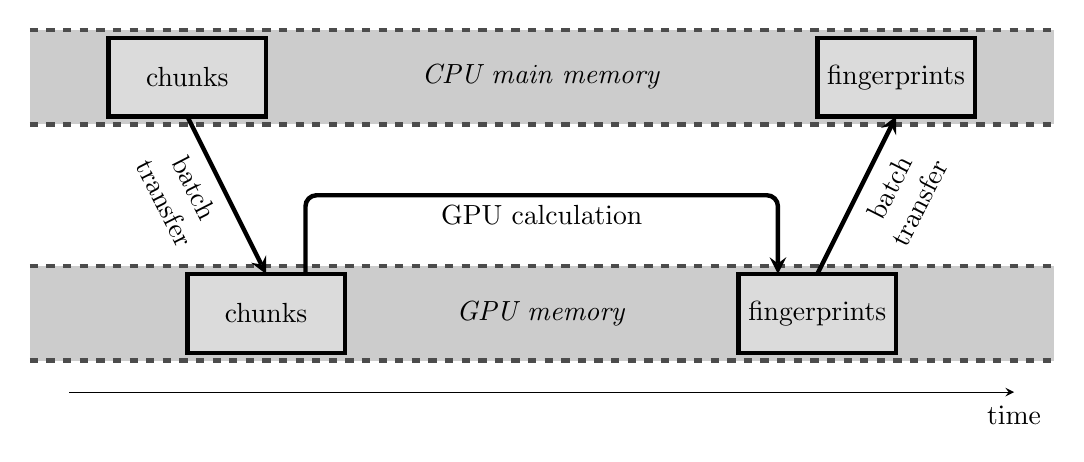
\begin{tikzpicture}
 \fill[fill=black!20, dashed] (0, -1.9) rectangle (13, -3.1);
 \fill[fill=black!20, dashed] (0, -4.9) rectangle (13, -6.1);
 \draw[ultra thick,dashed,color=black!70] (0,-1.9) -- (13,-1.9);
 \draw[ultra thick,dashed,color=black!70] (0,-3.1) -- (13,-3.1);
 \draw[ultra thick,dashed,color=black!70] (0,-4.9) -- (13,-4.9);
 \draw[ultra thick,dashed,color=black!70] (0,-6.1) -- (13,-6.1);
 
 \draw[ultra thick, fill=black!14] (1, -2) rectangle (3, -3);
 \draw[ultra thick, fill=black!14] (10, -2) rectangle (12, -3);
 \draw[ultra thick, fill=black!14] (2, -5) rectangle (4, -6);
 \draw[ultra thick, fill=black!14] (9, -5) rectangle (11, -6);
 \node at (2, -2.5) {chunks};
 \node at (11, -2.5) {fingerprints};
 \node at (3, -5.5) {chunks};
 \node at (10, -5.5) {fingerprints};
 \draw[ultra thick, -stealth] (2, -3)--(3, -5);
 \draw[ultra thick, -stealth] (10, -5)--(11, -3);
 \draw[ultra thick, rounded corners, -stealth] (3.5, -5)--(3.5, -4)--(9.5, -4)--(9.5, -5);
 \node at (6.5, -2.5) {\textit{CPU main memory}};
 \node at (6.5, -5.5) {\textit{GPU memory}};
 \node[below] at(6.5, -4) {GPU calculation};
 
 \node[rotate=-63] at (1.9,-4) {\parbox{0.5in}{\centering batch transfer}};
 \node[rotate=63] at (11.1,-4) {\parbox{0.5in}{\centering batch transfer}};
 
 \draw[-stealth] (0.5, -6.5) -- (12.5, -6.5);
 \node at (12.5, -6.8) {time};
 \end{tikzpicture}
%}

\caption{Illustrating data transfers between the CPU-side main memory and the GPU memory.  We use batching to reduce the number of CPU-GPU transfers.}
\label{fig:gpu-data}
\end{figure}

The benefits of offloading SHA1 calculation instead of chunking to the GPU are:
\begin{itemize}
\item The GPU hardware is not efficient for applications with intensive branch instructions or data synchronization since it is not allowable for the threads of the same thread block to concurrently jump to different branches~\cite{li2013a}.

\item The input size of chunking process is larger (chunking is the process which segments large data blocks into small, closely sized chunks). In our experimental configuration, we use a 96MB data block (as might arise in a deduplication data stream) to a chunking thread, which would be too large for a single GPU thread. Moreover, chunking is an inherently serial process, in that chunk boundaries influence one another. SHA1 calculation for the already-computed chunks is far simpler to parallelize since the chunks are of similar sizes, so the task sizes are better balanced.

\end{itemize}

\subsection{Balance between computation and I/O}

Data deduplication is both computationally intensive and I/O intensive.  With lazy deduplication, we reduce the I/O component (primarily fingerprint identification) to the extent that the computational component becomes the new bottleneck (primarily computing the chunks and calculating their fingerprints).  If we improve only one of these components (or even if we eliminate it entirely), Ahmdal's Law gives a theoretical limit on the benefit.

Figure~\ref{fig:balance-pie} shows the proportion of time spent on computation in lazy deduplication as we introduce GPU fingerprinting and multi-threaded chunking on the CPU. We use the FSLHomes~\cite{tarasov2012generating} (which we use for experiments; see Section~\ref{se:exp_det}) as an example. We use the data from Tables~\ref{tab:disk-bar}, ~\ref{tab:gpu} and Figure~\ref{fig:chunk-speed}. This figure shows the bottleneck stage in each optimizing step.

Using the lazy method, disk I/O is reduced. As a consequence, the identification component only takes 13\% of the deduplication time. Chunking and hashing consume larger proportions of the deduplication time, especially chunking which takes over half (53\%) of the entire time. So it is impossible for the overall throughput to exceed the chunking throughput, which is only 217MB/sec..

Tough fingerprinting takes less proportion of the time than chunking, it is one potential bottleneck. We offload the hash calculation to GPU, which doesn't wholly eliminate the fingerprinting component, but reduces it to 10\%.  Chunking remains the bottleneck, taking 74\% of the deduplication time. The throughput still can not exceed the chunking throughput.
So we use multiple CPU threads to perform chunking, dropping this component to 39\%. After that, the time spent on each stage is close and the system reaches a relative balance. This means that the CPU, GPU and the disk work simultaneously and the resources are relatively fully used.

The other two data sets (Vm and Src) also show similar trend.

\begin{figure}[htbp]
\centering
\resizebox{0.8\textwidth}{!}{
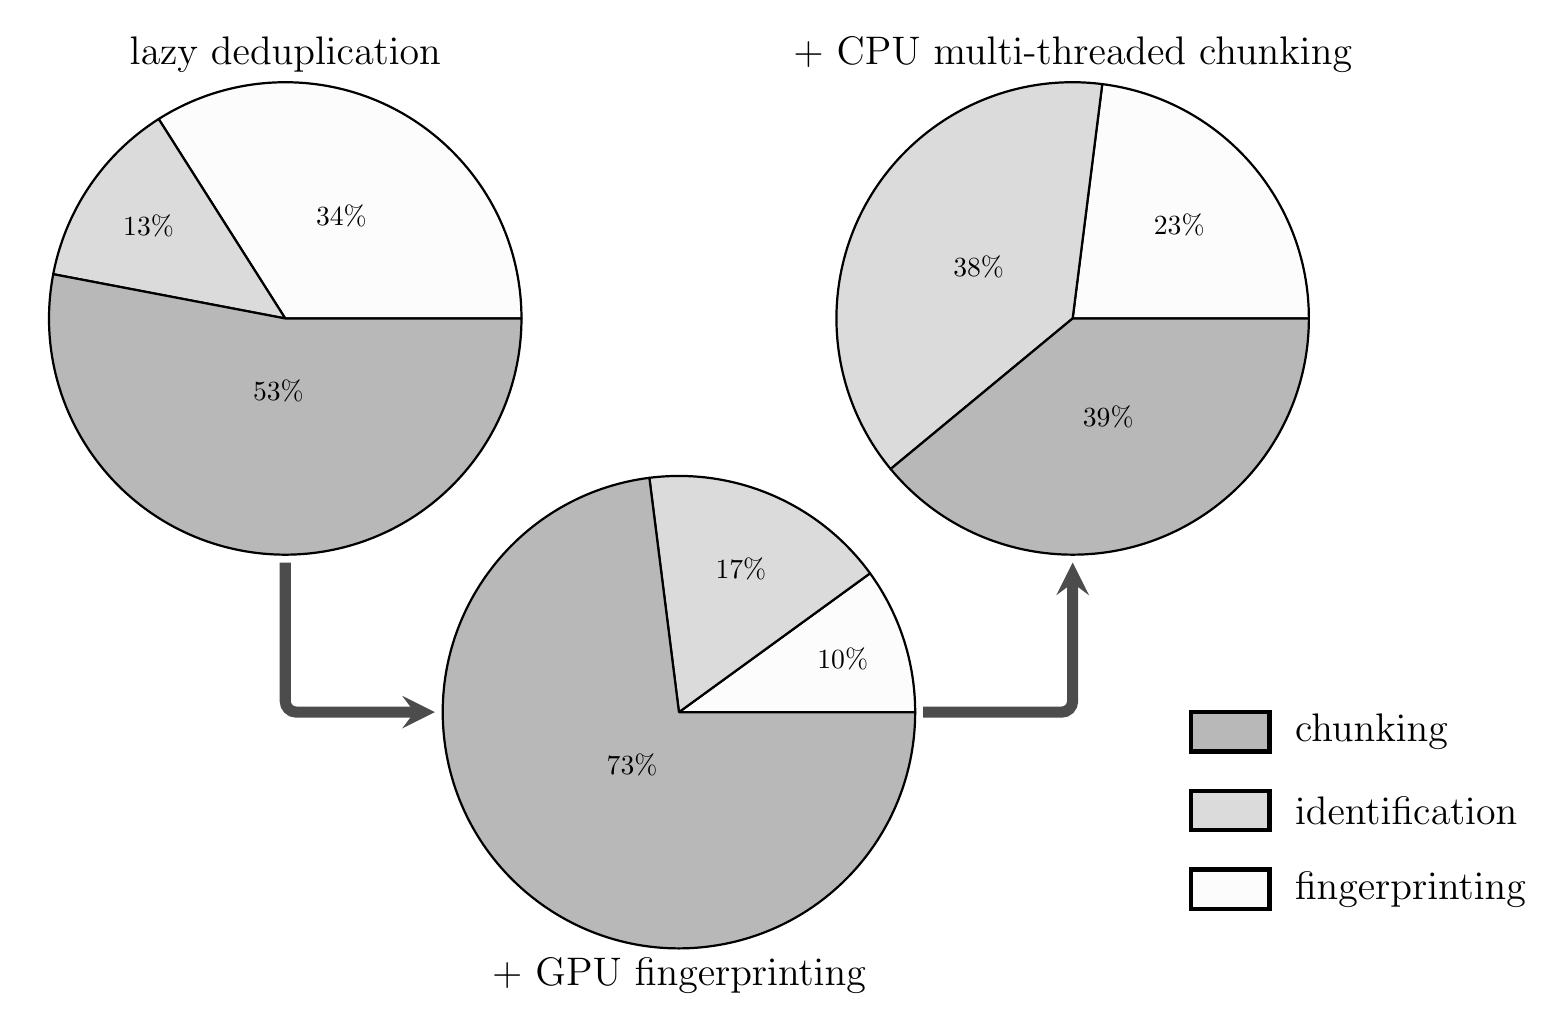
\begin{tikzpicture}
\pie[pos={-5,5}, color={black!1, black!14, black!28}]
{34/, 13/, 53/}
\node[below] at (-5, 8.7) {\Large lazy deduplication};

\pie[pos={0, 0}, color={black!1, black!14, black!28}]
{10/, 17/, 73/}
\node[below] at (0, -3) {\Large + GPU fingerprinting};

\pie[pos={5,5}, color={black!1, black!14, black!28}]
{23/, 38/, 39/}
\node[below] at (5, 8.7) {\Large + CPU multi-threaded chunking};

\draw[line width=4pt, -stealth, color=black!70, rounded corners] (-5, 1.9) |- (-3.1, 0);
\draw[line width=4pt, -stealth, color=black!70, rounded corners] (3.1, 0) -| (5, 1.9);

%legend here
\draw[ultra thick, fill=black!1]  (6.5, -2) rectangle (7.5, -2.5);
\draw[ultra thick, fill=black!14] (6.5, -1) rectangle (7.5, -1.5);
\draw[ultra thick, fill=black!28] (6.5, -0) rectangle (7.5, -0.5);
\node[right] at (7.7 , -2.25) {\Large fingerprinting};
\node[right] at (7.7 , -1.25) {\Large identification};
\node[right] at (7.7 , -0.25) {\Large chunking};

\end{tikzpicture}
}

\caption{How the execution time balance changes as we introduce (a) GPU fingerprinting and (b) CPU multi-thread chunking into lazy deduplication.}
\label{fig:balance-pie}
\end{figure}


\section{Prototype implementation}
\label{sec:prototype}

\subsection{Disk management}

The three main on-disk components are: data, metadata, and the hash table, which we describe in this section.  The disk layout for metadata and the on-disk hash table is illustrated in Figure~\ref{fig:data-layout}.

\begin{figure}[htbp]
  \begin{center}
  \includegraphics[width=0.6\textwidth]{data-layout}
  \end{center}
  \caption{Disk layout for metadata and the on-disk hash table in lazy deduplication.  Here ``fps'' denotes a collection of fingerprints.  The storage of data is not shown.}
  \label{fig:data-layout}
\end{figure}


\subsection{Data layout}

\subsubsection{Data}

Data are stored in a log-structured layout, divided into \emph{data segments} of fixed maximum size.  Incoming chunks, if found to be unique (i.e., have not been seen previously), are added to the ``current'' data segment, which when full, is added to the disk.  Data segments are \emph{chained}, i.e., each data segment has a pointer to the next data segment.

\subsubsection{Metadata}

Pointers (8-byte offset; 4-byte length) to the data chunks together with the fingerprints are stored in the metadata in a log-structured layout, divided into \emph{metadata segments} of fixed maximum size (for simplicity, we choose the same maximum size as for data).  For each incoming fingerprint, whether unique or not, an entry is stored to the location of the corresponding chunk in the data.  We use metadata to keep track of the temporal order in which chunks arrive. The metadata stores the information about which chunks a file consists of; they are small and there are duplicate metadata entries.

\subsubsection{On-disk hash table}

When one of the hash buckets in the buffer is full, the fingerprints in it are looked up as a batch on disk. The on-disk fingerprints are stored in the on-disk hash table.  Fingerprints are stored together with a pointer to a corresponding metadata entry.  On-disk hash buckets are chained together to facilitate on-disk lookups of fingerprints. For each unique chunk, after its metadata entry is inserted, one hash table entry is added to the corresponding bucket. An entry consists of the fingerprint, an 8-byte pointer to show the metadata entry position, and a pair (8-byte offset, 4-byte length) giving the chunk information. Entries in the bucket are stored one by one until the bucket is full.

We implement a lazy deduplication prototype using the CDC chunking method~\cite{policroniades2004alternatives} with a $4$KB target. The Rabin Hash algorithm is used to calculate the signature in the sliding window. We use SHA1 to calculate the fingerprints.


In our implementation, the cache is organized into a hash table with collision lists and a LRU eviction policy.  We bypass the file system cache to avoid its impact on the experimental results.


\subsection{Deduplication pipeline}

We use multiple CPU threads and a GPU to accelerate chunking and fingerprinting. The system creates $8$ chunking threads (equal to the the number of logical CPU processors on our platform), each for processing data in $96$MB blocks. On fingerprint calculation, the system transfers batches of $4096$ chunks to the GPU (to closely match the GPU's $3584$ cores). The GPU assigns a thread to each data chunk in a batch to calculate its fingerprint, and then transfers the batch of fingerprints from the GPU to the main memory.  Identification picks out the redundant fingerprints, which are buffered for later processing. Though all the stages except fingerprinting run on the CPU, only chunking is computationally intensive. Fingerprint identification is instead disk-I/O-intensive.

Though multi-threading and using a GPU can improve the chunking and hash calculation procedures directly, they can also perform these tasks in parallel to one another via pipelining. Figure~\ref{fig:pipeline} illustrates how each stage executes in parallel. In our deduplicaton implementation, we divide the process into 4 stages, namely chunking, fingerprinting, identification, and storage\footnote{In our deduplicaton implementation, we don't actually store the chunks, so it consumes no CPU resources.}.  Importantly, these components are approximately time-balanced (see Figure~\ref{fig:balance-pie}), which helps pipelining to avoid idle time.  By organizing the workload onto three devices, the CPU, GPU, and disk, which can operate simultaneously, the time spent can overlap with each other. 

\begin{figure}[htbp]
\centering
\resizebox{0.7\textwidth}{!}{
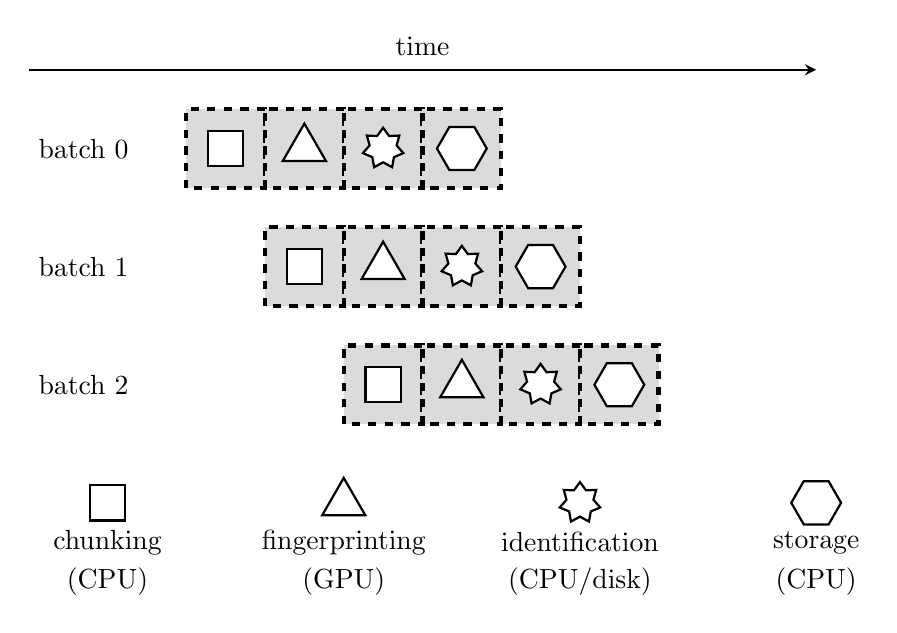
\begin{tikzpicture}
 \draw[-stealth, thick] (0, 7.5) to (10, 7.5);
 \node at (5, 7.8) {time};

 \draw[ultra thick, fill=black!14, dashed] (2, 6) rectangle (3, 7);
 \node[thick,regular polygon,regular polygon sides=4,draw,inner sep=0pt,minimum width=18pt,fill=white] at (2.5,6.5) {};
 \draw[ultra thick, fill=black!14, dashed] (3, 6) rectangle (4, 7);
 \node[thick,regular polygon,regular polygon sides=3,draw,inner sep=0pt,minimum width=18pt,fill=white] at (3.5,6.5) {};
 \draw[ultra thick, fill=black!14, dashed] (4, 6) rectangle (5, 7);
 \node[thick,star,star points=7,draw,inner sep=0pt,minimum width=15pt,fill=white] at (4.5,6.5) {};
 \draw[ultra thick, fill=black!14, dashed] (5, 6) rectangle (6, 7);
 \node[thick,regular polygon,regular polygon sides=6,draw,inner sep=0pt,minimum width=18pt,fill=white] at (5.5,6.5) {};

 
 \draw[ultra thick, fill=black!14, dashed] (3, 4.5) rectangle (4, 5.5);
 \node[thick,regular polygon,regular polygon sides=4,draw,inner sep=0pt,minimum width=18pt,fill=white] at (3.5,5) {};
 \draw[ultra thick, fill=black!14, dashed] (4, 4.5) rectangle (5, 5.5);
 \node[thick,regular polygon,regular polygon sides=3,draw,inner sep=0pt,minimum width=18pt,fill=white] at (4.5,5) {};
 \draw[ultra thick, fill=black!14, dashed] (5, 4.5) rectangle (6, 5.5);
 \node[thick,star,star points=7,draw,inner sep=0pt,minimum width=15pt,fill=white] at (5.5,5) {};
 \draw[ultra thick, fill=black!14, dashed] (6, 4.5) rectangle (7, 5.5);
 \node[thick,regular polygon,regular polygon sides=6,draw,inner sep=0pt,minimum width=18pt,fill=white] at (6.5,5) {};

 
 \draw[ultra thick, fill=black!14, dashed] (4, 3) rectangle (5, 4);
 \node[thick,regular polygon,regular polygon sides=4,draw,inner sep=0pt,minimum width=18pt,fill=white] at (4.5,3.5){};
 \draw[ultra thick, fill=black!14, dashed] (5, 3) rectangle (6, 4);
 \node[thick,regular polygon,regular polygon sides=3,draw,inner sep=0pt,minimum width=18pt,fill=white] at (5.5,3.5) {};
 \draw[ultra thick, fill=black!14, dashed] (6, 3) rectangle (7, 4);
 \node[thick,star,star points=7,draw,inner sep=0pt,minimum width=15pt,fill=white] at (6.5,3.5) {};
 \draw[ultra thick, fill=black!14, dashed] (7, 3) rectangle (8, 4);
 \node[thick,regular polygon,regular polygon sides=6,draw,inner sep=0pt,minimum width=18pt,fill=white] at (7.5,3.5) {};

 
 \node[thick,regular polygon,regular polygon sides=4,draw,inner sep=0pt,minimum width=18pt,fill=white] at (1,2){};
 \node at (1, 1.5) {chunking};
 \node at (1, 1) {(CPU)};
 \node[thick,regular polygon,regular polygon sides=3,draw,inner sep=0pt,minimum width=18pt,fill=white] at (4,2) {};
 \node at (4, 1.5) {fingerprinting};
 \node at (4, 1) {(GPU)};
 \node[thick,star,star points=7,draw,inner sep=0pt,minimum width=15pt,fill=white] at (7,2) {};
 \node at (7, 1.5) {identification};
 \node at (7, 1) {(CPU/disk)};
 \node[thick,regular polygon,regular polygon sides=6,draw,inner sep=0pt,minimum width=18pt,fill=white] at (10,2) {};
 \node at (10, 1.5) {storage};
 \node at (10, 1) {(CPU)};
 
 \node[right] at (0, 6.5) {batch 0};
 \node[right] at (0, 5) {batch 1};
 \node[right] at (0, 3.5) {batch 2};

 \end{tikzpicture}
 }
 \caption{Illustrating how pipelining can be used to improve computation in lazy deduplication. Batches are able to processed in parallel using separate CPU threads.}
\label{fig:pipeline}
\end{figure}



\section{Performance evaluation}
\label{sec:evaluation}

We measure \emph{deduplication time} which we define as,  for a given data set, the time it takes to classify pre-computed fingerprints as ``unique'' or ``duplicate''.

When measuring deduplication time, the process is simulated, in that we do not include the time for chunking, fingerprinting, and writing data chunks to disk. In this way, we focus on fingerprint lookup performance.  Reading the data from disk and writing the unique data chunks to disk will affect deduplication performance, but disk storage methods are instead chosen to optimize the system's online performance, and go beyond the scope of this article. We compare the deduplication time of the lazy method to the eager method.

We also investigate \emph{deduplication throughput}, where we include chunking and fingerprint calculation time (except for the FSLHomes data set, where we only have access to fingerprints).  Note that the GPU and CPU parallelism is used to speed up chunking and fingerprint calculation (except for FSLHomes).


Each experiment runs $10$ times and we give the average results. The errors encountered were consistently negligible (typically around $1\%$) and are omitted.

\subsection{Experimental details}\label{se:exp_det}

To compare eager and lazy deduplication as fairly as possible, they are both assigned a fixed $1$GB Bloom filter, and we allocate them the same amount of memory ($256$MB in two experiments). For eager deduplication, the memory is fully allocated to the cache. For lazy deduplication, half of the memory is reserved for the buffer (storing both fingerprints and their corresponding chunks), and the remainder is allocated to the cache.  The lazy method always has BFT set to $32$ except for the test to evaluate the influence of BFT.

Table~\ref{tab:platform} lists the platform details. The operating system was installed on one HDD (HDD-OS). SSD-M and HDD-M respectively refer to the SSD and HDD used to store metadata and the on-disk hash table. Except for the HDD vs.\ SSD throughput performance test, we always perform deduplication on the SSD. 

\begin{table}[htbp]
    \centering
    \begin{tabular}{lr}
        \toprule
        CPU   & Intel(R) Core(TM) i7-3770 @3.40GHz \\
        Memory & $4 \times$ (CORSAIR) Vengeance DDR$3$ $1600$ $8$GB \\
        GPU & GeForce Titan (NVIDIA Corporation Device 1005 (rev.\ a1)) \\
        HDD-OS & WDC WD20EARX-07PASB0 $2$TB $64$MB IntelliPower \\
        HDD-M & WDC WD5000AADS-00S9B0 $500$GB $16$MB 7200rpm \\
        SSD-M & OCZ-AGILITY3 $120$GB \\
        OS & CentOS release 6.3 (Final) \\
        Kernel & Linux-2.6.32-279.22.1.e16.x86\_64 \\
        \bottomrule
    \end{tabular}
    \caption{Platform details.}
    \label{tab:platform}
\end{table}

Table~\ref{tab:data} lists the details of the three data sets we used in our experiments:
\begin{itemize}
 \item \textit{Vm} refers to pre-made VM disk images from VMware's Virtual Appliance Marketplace\footnote{\url{http://www.thoughtpolice.co.uk/vmware/}}, which is used by Jin~\cite{jin2009the} to explore the effectiveness of deduplication on virtual machine disk images.
 \item \textit{Src} refers to the software sources of ArchLinux, CentOS, Fedora, Gentoo, Linux Mint, and Ubuntu at 5 June 2013, collected from the Linux software source server at Nankai University.
 \item \textit{FSLHomes}\footnote{\url{http://tracer.filesystems.org/traces/fslhomes/2014/}} is published by the File system and Storage Lab (FSL) at Stony Brook University~\cite{tarasov2012generating}. It contains snapshots of students' home directories. The files consist of source code, binaries, office documents, and virtual machine images.  We collect the data in $7$-day intervals from the year 2014, simulating weekly backups. If the data on one date is not available, we choose the closest following available date.  These are combined into the FSLHomes data set.
\end{itemize}

Unlike Vm and Src, FSLHomes directly gives the fingerprints, so chunking cannot be performed. FSLHomes has a large amount of redundant data.

\begin{table}[htbp]
\centering
{
\begin{tabular}{lrr}
\toprule
 & total size & duplication \\
\cmidrule(lr){2-2}\cmidrule(lr){3-3}
Vm & $220.85$GB & 35\% \\
Src & $434.88$GB & 19\% \\
FSLHomes & $3.58$TB & 91\% \\
\bottomrule
\end{tabular}
}
\caption{Data sets used for the experiments along with the proportion of duplicate data.}
\label{tab:data}
\end{table}

\subsection{Deduplication time}

Table~\ref{tab:dedup-time} gives the deduplication times for eager and lazy deduplication on the three data sets (Vm, Src, and FSLHomes).  With the lazy method, deduplication time is reduced by $46\%$, $53\%$, and $32\%$ on Vm, Src, and FSLHomes, respectively.  This experiment consistently shows that lazy deduplication is faster than eager deduplication.

\begin{table}[htp]
\centering
\begin{tabular}{lrrr}
\toprule
 & Vm & Src & FSLHomes \\
\cmidrule(lr){2-2}\cmidrule(lr){3-3}\cmidrule(lr){4-4}
eager & $282$ & $476$ & $5824$ \\
lazy  & $151$ & $226$ & $3939$ \\
\bottomrule
\end{tabular}
\caption{Deduplication time (sec.) for lazy deduplication and eager deduplication.}
\label{tab:dedup-time}
\end{table}


\subsection{Buffer cycle effectiveness}

We test the effectiveness of the lazy fingerprint buffer strategy (which utilizes buffer cycles and ranks) by comparing it with a \emph{buffer-exhausting} strategy, which instead compares all the fingerprints in the buffer area with the prefetched ones to find as many duplicate fingerprints as possible.  The results are shown in Table~\ref{tab:list-lookup-result}.  During the test, we disable pre-lookup, which could interfere with the strategies' effectiveness.  Generally, the buffer cycle strategy has a better performance than the buffer-exhausting strategy.

\begin{table}[htp]
\centering
\begin{tabular}{lrrrrrr}
\toprule
Data set & \multicolumn{2}{c}{Vm} & \multicolumn{2}{c}{Src} & \multicolumn{2}{c}{FSLHomes} \\
\cmidrule(lr){2-3} \cmidrule(lr){4-5} \cmidrule(lr){6-7}
Method & lazy$^*$ & exh.$^*$ & lazy$^*$ & exh.$^*$ & lazy$^*$ & exh.$^*$ \\
\midrule
cache lookup & $11$ & $83$ & $9$ & $50$ & $279$ & $5474$ \\
on-disk lookup & $41$ & $32$ & $58$ & $37$ & $19464$ & $18398$ \\
prefetching & $74$ & $60$ & $82$ & $69$ & $1681$ & $1882$ \\
other & $74$ & $63$ & $106$ & $90$ & $2544$ & $2720$ \\
\midrule
total & $199$ & $237$ & $255$ & $246$ & $23969$ & $28474$ \\
\bottomrule
\end{tabular}
\caption{Deduplication time (sec.) for the lazy deduplication (lazy$^*$) and the buffer-exhausting strategy (exh.$^*$). $^*$Pre-lookup has been disabled.}
\label{tab:list-lookup-result}
\end{table}

Due to its design, the buffer-exhausting strategy has the following properties (compared with the lazy buffering strategy):
\begin{itemize}
 \item It finds more fingerprints in the cache, but has a low cache hit rate.  As a result, the buffer-exhausting method saves $5\%$ to $36\%$ of the time spent on on-disk lookup, while the time spent on cache lookups increases by a factor of $6$ to $20$.
 
 \item Since Vm and FSLHomes have more redundant data, the cache lookup time occupies a greater fraction of the total time.  In Src there are relatively few duplicate chunks, so the increase of cache lookup in going from lazy to buffer-exhausting does not make the performance significantly worse due to the disk access savings.

 \item It prefetches less often, since prefetching is triggered after a fingerprint is found on the disk.
\end{itemize}

\subsection{Pre-lookup and post-lookup}

We test the performance of lazy deduplication with both pre-lookup and post-lookup vs.\ with post-lookup alone.  The results are shown in Table~\ref{tab:two-stage-result}.

\begin{table}[htp]
\centering
\begin{tabular}{lrrrrrr}
\toprule
Data set & \multicolumn{2}{c}{Vm} & \multicolumn{2}{c}{Src} & \multicolumn{2}{c}{FSLHomes} \\
\cmidrule(lr){2-3} \cmidrule(lr){4-5} \cmidrule(lr){6-7}
% Method & bi. & sec. & bi. & sec. & bi. & sec. \\
Method & lazy & lazy$^*$ & lazy & lazy$^*$ & lazy & lazy$^*$ \\
\midrule
on-disk lookup & $20$ & $41$ & $45$ & $58$ & $1639$ & $19464$ \\
prefetching & $60$ & $74$ & $68$ & $82$ & $655$ & $1681$ \\
pre-lookup & $8$ & --- & $14$ & --- & $462$ & ---\\
post-lookup & $5$ & $11$ & $5$ & $9$ & $133$ & $279$ \\
other & $69$ & $95$ & $106$ & $124$ & $1049$ & $2544$ \\
\midrule
total & $152$ & $199$ & $227$ & $255$ & $3939$ & $23969$ \\
\bottomrule
\end{tabular}
\caption{Deduplication time (sec.) with both pre-lookup and post-lookup (lazy) and with pre-lookup disabled (lazy$^*$).}
\label{tab:two-stage-result}
\end{table}

Fingerprints found during pre-lookup are not searched for on disk and so prefetching is not triggered.  Thus, we observe that the time spent on on-disk fingerprint lookup and prefetching is reduced.  Using pre-lookup reduces deduplication time by $24\%$ for Vm, $11\%$ for Src, and $84\%$ FSLHomes (where the majority of time spent was on on-disk lookup).

Table~\ref{tab:hit-rate} lists the cache hit rates for pre-lookup and post-lookup in lazy deduplication.  (The post-lookup cache hit rate is measured without disabling pre-lookup.) Pre-lookup is used on the fingerprints that pass through the Bloom filter, identifying a significant proportion of such fingerprints.  We see that Vm results in a higher pre-lookup cache hit rate and Src and FSLHomes result in a higher post-lookup cache hit rate.  For all three data sets, both pre-lookup and post-lookup result a significant reduction in disk accesses.

\begin{table}[htbp]
\centering
\begin{tabular}{lcc}
\toprule
& pre-lookup & post-lookup \\
\cmidrule(lr){2-2}\cmidrule(lr){3-3}
Vm & $ 74\%$ & $26\%$ \\
Src & $43\%$ & $57\%$ \\
FSLHomes & $45\%$ & $55\%$ \\
\bottomrule
\end{tabular}
\caption{Cache hit rates for pre-lookup and post-lookup in lazy deduplication.}
\label{tab:hit-rate}
\end{table}

\subsection{Buffer fingerprint threshold}

The buffer fingerprint threshold (BFT) is the primary factor affecting the performance of lazy deduplication. Figure~\ref{fig:bft} plots the deduplication time of lazy deduplication as the buffer fingerprint threshold (BFT) varies from $4$ to $60$. During the test, the total memory size of the buffer and the cache is set to $256$MB, so if the buffer needs more memory due to a larger BFT, there will be less memory for the cache. When limiting the memory size, $64$ is the largest BFT the system can reach. Leaving a small part of memory for the cache, we set the maximum BFT as 60 in the experiment.

\begin{figure}
\centering

\includegraphics[width=0.8\columnwidth]{bft-vm}
\\[0.5em]

\includegraphics[width=0.8\columnwidth]{bft-src}
\\[0.5em]

\includegraphics[width=0.8\columnwidth]{bft-fslhomes}
\\[0.5em]
\caption{Deduplication time for lazy deduplication as the buffer fingerprint threshold varies.}
\label{fig:bft}
\end{figure}

Experimental results show a significant impact of BFT on deduplication time. When BFT is small, the on-disk fingerprint lookup time dominates the overall time. As BFT increases, the on-disk lookup time drops quickly, and the deduplication time decreases. However, when BFT becomes large, both the on-disk lookup time and prefetching time begins to increase due to the smaller cache size. There is a ``sweet spot'' for each data set. In our experiments, they are all close to 32, so we choose 32 as the default BFT.

\subsection{Disk Access Time}

Here we test the on-disk fingerprint lookup time and fingerprint prefetching time, together with the deduplication time, for eager and lazy deduplication, the results of which are shown in Table~\ref{tab:disk-bar}.

\begin{table}[htp]
\centering
\begin{tabular}{lrrrrrr}
\toprule
Data set & \multicolumn{2}{c}{Vm} & \multicolumn{2}{c}{Src} & \multicolumn{2}{c}{FSLHomes} \\
\cmidrule(lr){2-3} \cmidrule(lr){4-5} \cmidrule(lr){6-7}
Method & eager & lazy & eager & lazy & eager & lazy \\
\midrule
on-disk lookup & $176$ & $20$ & $325$ & $45$ & $4598$ & $1639$ \\
prefetching & $46$ & $60$ & $52$ & $68$ & $298$ & $655$ \\
other & $59$ & $71$ & $99$ & $113$ & $928$ & $1645$ \\
\midrule
total disk access & $222$ & $80$ & $377$ & $113$ & $4896$ & $2294$ \\
\midrule
total dedup. & $282$ & $151$ & $476$ & $226$ & $5824$ & $3939$\\
\bottomrule
\end{tabular}
\caption{Disk access time (sec.) for eager and lazy deduplication.}
\label{tab:disk-bar}
\end{table}

The time consumed by on-disk lookups is reduced by $64\%$ to $89\%$. As a result, its proportional contribution to the total time is also significantly reduced: in eager deduplication, on-disk fingerprint lookup alone takes over $62\%$ to $84\%$ of the total time, which drops to $13\%$ to $42\%$ using the lazy method.  This is precisely what lazy deduplication was designed to achieve.


\subsection{Bloom filter size}\label{se:Bloom}

The Bloom filter effectively filters out the unique fingerprints. However, as the data size grows, it becomes less effective in deduplication due to more false positives.  Here we explore how the size of the Bloom filer impacts the deduplication performance.  A smaller-sized Bloom filter will give rise to more frequent false positives much like a data set with more unique data.  Table~\ref{tab:bloom-filter} lists run time measurements showing the time spent on each component and the improvement in terms of speedup in deduplication time.

\begin{table}[htp]
\centering
\begin{tabular}{llrrrrrr}
\toprule
\multirow{2}{*}{Bf size (MB)} & Data sets& \multicolumn{2}{c}{Vm} & \multicolumn{2}{c}{Src} & \multicolumn{2}{c}{FSLHomes}\\
\cmidrule(lr){2-2} \cmidrule(lr){3-4} \cmidrule(lr){5-6} \cmidrule(lr){7-8}
 &Method & eager & lazy & eager & lazy & earger & lazy\\
\midrule

\multirow{5}{*}{1024} & false positive rate & \multicolumn{2}{c}{$0.00$} & \multicolumn{2}{c}{$0.00$} & \multicolumn{2}{c}{$1.14\times10^{-9}$} \\
& on-disk lookup (sec.)& $176$ & $20$ & $325$ & $45$ & $4598$ & $1639$ \\
& prefetching (sec.) & $46$ & $60$ & $52$ & $68$ & $298$ & $655$  \\
& total dedup. (sec.) & $282$ & $151$ & $476$ & $226$ & $5824$ & $3939$ \\
& throughput speedup & \multicolumn{2}{c}{$\times 1.9$} & \multicolumn{2}{c}{$\times 2.1$} & \multicolumn{2}{c}{$\times 1.5$} \\

\cmidrule(lr){1-1} \cmidrule(lr){2-2} \cmidrule(lr){3-4} \cmidrule(lr){5-6} \cmidrule(lr){7-8}
\multirow{5}{*}{512} & false positive rate & \multicolumn{2}{c}{$0.00$} & \multicolumn{2}{c}{$5.57\times 10^{-7}$} & \multicolumn{2}{c}{$3.08\times 10^{-8}$} \\
& on-disk lookup (sec.)& $175$ & $21$ & $324$ & $46$ & $4613$ & $1686$ \\
& prefetching (sec.) & $46$ & $61$ & $52$ & $69$ & $299$ & $667$  \\
& total dedup. (sec.) & $280$ & $152$ & $476$ & $228$ & $5824$ & $3968$ \\
& throughput speedup & \multicolumn{2}{c}{$\times 1.8$} & \multicolumn{2}{c}{$\times 2.1$} & \multicolumn{2}{c}{$\times 1.5$} \\

\cmidrule(lr){1-1} \cmidrule(lr){2-2} \cmidrule(lr){3-4} \cmidrule(lr){5-6} \cmidrule(lr){7-8}
\multirow{5}{*}{256} & false positive rate & \multicolumn{2}{c}{$0.00$} & \multicolumn{2}{c}{$3.92\times 10^{-5}$} & \multicolumn{2}{c}{$1.17\times 10^{-6}$} \\
& on-disk lookup (sec.)& $175$ & $21$ & $335$ & $47$ & $4620$ & $1694$ \\
& prefetching (sec.) & $46$ & $61$ & $52$ & $69$ & $298$ & $669$ \\
& total dedup. (sec.) & $278$ & $152$ & $488$ & $229$ & $5825$ & $4003$ \\
& throughput speedup & \multicolumn{2}{c}{$\times 1.8$} & \multicolumn{2}{c}{$\times 2.1$} & \multicolumn{2}{c}{$\times 1.5$} \\

\cmidrule(lr){1-1} \cmidrule(lr){2-2} \cmidrule(lr){3-4} \cmidrule(lr){5-6} \cmidrule(lr){7-8}
\multirow{5}{*}{128} & false positive rate & \multicolumn{2}{c}{$2.69\times 10^{-6}$} & \multicolumn{2}{c}{$1.56\times 10^{-3}$} & \multicolumn{2}{c}{$4.12\times 10^{-5}$} \\
& on-disk lookup (sec.)& $176$ & $21$ & $736$ & $67$ & $5077$ & $1752$ \\
& prefetching (sec.) & $46$ & $61$ & $52$ & $70$ & $299$ & $692$  \\
& total dedup. (sec.) & $281$ & $153$ & $908$ & $253$ & $6314$ & $4055$\\
& throughput speedup & \multicolumn{2}{c}{$\times 1.8$} & \multicolumn{2}{c}{$\times 3.6$} & \multicolumn{2}{c}{$\times 1.6$} \\

\cmidrule(lr){1-1} \cmidrule(lr){2-2} \cmidrule(lr){3-4} \cmidrule(lr){5-6} \cmidrule(lr){7-8}
\multirow{5}{*}{64} & false positive rate & \multicolumn{2}{c}{$1.14\times 10^{-4}$} & \multicolumn{2}{c}{$3.31\times 10^{-2}$} & \multicolumn{2}{c}{$9.20\times 10^{-4}$} \\
& on-disk lookup (sec.)& $185$ & $21$ & $9553$ & $660$ & $15421$ & $2953$ \\
& prefetching (sec.) & $46$ & $61$ & $52$ & $79$ & $310$ & $1081$  \\
& total dedup. (sec.) & $290$ & $153$ & $10156$ & $886$ & $17149$ & $5785$ \\
& throughput speedup & \multicolumn{2}{c}{$\times 1.9$} & \multicolumn{2}{c}{$\times 11$} & \multicolumn{2}{c}{$\times 3.0$} \\

\cmidrule(lr){1-1} \cmidrule(lr){2-2} \cmidrule(lr){3-4} \cmidrule(lr){5-6} \cmidrule(lr){7-8}
\multirow{5}{*}{32} & false positive rate & \multicolumn{2}{c}{$3.36\times 10^{-3}$} & \multicolumn{2}{c}{$2.62\times 10^{-1}$} & \multicolumn{2}{c}{$9.21\times 10^{-3}$} \\
& on-disk lookup (sec.)& $410$ & $35$ & $100369$ & $6292$ & $113334$ & $10915$\\
& prefetching (sec.) & $46$ & $63$ & $54$ & $115$ & $338$ & $1430$ \\
& total dedup. (sec.) & $527$ & $171$ & $105398$ & $6866$ & $119855$ & $14571$\\
& throughput speedup & \multicolumn{2}{c}{$\times 3.1$} & \multicolumn{2}{c}{$\times 15$} & \multicolumn{2}{c}{$\times 8.2$} \\

\bottomrule
\end{tabular}
\caption{Impact of the Bloom filter size on false positives; the speedup is for lazy vs.\ eager.}
\label{tab:bloom-filter}
\end{table}

When the size of Bloom filter is sufficiently large, the false positive rate is low, so there are fewer disk accesses, so the difference between eager and lazy is narrow.  With a smaller Bloom filter, we have a higher false positive rate and consequently more disk accesses.  The time spent on on-disk fingerprint lookup increases with the growth of the false positive rate for both eager and lazy methods as both need to search for the fingerprints in the case of a cache miss.  However, since the lazy method merges on-disk lookup, it takes much less time, so it can better handle situations where the Bloom filter has a large number of false positives.  

Due to its small data size, a substantial false positive rate does not appear on Vm until we cut the size of Bloom filter to 128MB. Though FSLHomes has a much larger total size than Src, it has a similar unique data size (Src: 352GB, compared to FSLHomes: 330GB). Src has far fewer duplicate fingerprints, so Src shows higher false positive rate.

In the eager method, the prefetching time does not increase with the false positive rate. This is because when a unique fingerprint is misclassified by the Bloom filter, the eager method just searches for it on the disk, which only introduce addition disk I/O for on-disk fingerprint lookup. As the fingerprint will not be found on the disk, prefetching is not triggered, so the prefeching time does not change.  However, in the lazy method, the prefetching time increases with the false positive rate. Since we buffer the fingerprints, if there are many unique fingerprints in the buffer, the true duplicates have to wait for slots. As a result, duplicate fingerprints are more sparsely spread throughout the buffer cycles, and fewer duplicate fingerprints are found after prefetching is triggered.  This results in prefetching being called more often, and a greater prefetching time.

Nevertheless, even with an increasing prefetching time, the lazy method is still beneficial due to the reduction of costly on-disk fingerprint lookups. For example, when the size of Bloom filter is set to 32MB, the lazy method can get a $\times 15$ improvement compared with the eager method on Src (despite prefetching time doubling in going from eager to lazy).


\subsection{Parallel computation}

We vary the number of threads from 1 to 8 and test the throughput of chunking. Figure~\ref{fig:chunk-speed} shows the speedup. The speed grows approximately linearly as the number of threads increases from 1 to 4. However, only a minor improvement in throughput is noticeable as the number of threads increases from 4 to 8, due to the CPU having 4 physical cores (supporting 8 logical processors). We still see an improvement from 4 threads to 8 threads, so we use 8 threads when testing the overall throughput.

\begin{figure}[htp]
\centering

\includegraphics[width=0.8\columnwidth]{chunk-speed}

\caption{Chunking throughput with different number of threads.}
\label{fig:chunk-speed}
\end{figure}

We use a GPU to accelerate fingerprinting (SHA1 hash calculation) and Table~\ref{tab:gpu} shows the improvement. We find that SHA1 on the GPU is 4.6 times faster than a single thread on CPU.

\begin{table}[htp]
\centering
\begin{tabular}{lrr}
\toprule
device & CPU (serial) & GPU \\
\cmidrule(lr){1-1} \cmidrule(lr){2-2} \cmidrule(lr){3-3}
throughput (MB/sec.) & $338$ & $1563$ \\
\bottomrule
\end{tabular}
\caption{GPU SHA1 speedup.}
\label{tab:gpu}
\end{table}


\subsection{Throughput}

Here we compare the throughput of lazy deduplication and eager deduplication on our SSD and HDD.  For Vm and Src, we calculate the throughput (from the start) at $20$GB intervals throughout the deduplication process.  For FSLHomes, we calculate the throughput at the end of each ``round'', where a round comprises the data from one weekly backup.  Since we only have the fingerprints for FSLHomes, we estimate the throughput where each fingerprint represents a $4$KB chunk.  Both eager and lazy deduplication utilize the GPU and CPU parallelism in the same way, but this is only relevant for the Vm and Src data sets.

Figure~\ref{fig:overall-SSD} shows the experimental results on our SSD. We see that lazy deduplication gives an improvement in the final throughput over eager deduplication of $80\%$, $65\%$, and $46\%$ for Vm, Src, and FSLHomes, respectively.  The lazy method achieves a greater throughput improvement vs.\ the eager method on Vm than Src since Src has less duplication, resulting in fewer on-disk lookups.

For Vm and Src, in the early stages, there are few fingerprints stored on disk, so looking up fingerprints does not require much disk I/O and throughput is limited by chunking. As more duplicate chunks arrive, the throughput drops as the system needs more disk I/O to find these duplicate chunks.

On FSLHomes, we see the overall throughput of the lazy method is $52\%$ higher than the eager method on the SSD. In the first round, as there are initially few duplicate chunks, the deduplication does not make many disk accesses, resulting in higher throughput than the other rounds.

For Vm and Src, duplicate data arise in various places in the data stream, which results in unstable throughput. We see a drop in throughput when there are many duplicates in the data stream as this results in more on-disk lookups.  For FSLHomes, as the duplicate chunks distribute evenly in each round of backup, we only see a slight change in throughput between adjacent backup rounds.

The results on our HDD are shown in Figure~\ref{fig:overall-HDD}. The improvements in the final throughput over eager are $150\%$, $119\%$, and  $79\%$ for Vm, Src, and FSLHomes, respectively. On HDD, The throughput is initially limited by chunking, but as the procedure goes on, on-disk fingerprint lookup becomes the bottleneck. For Vm and Src, the overall throughput on the HDD is limited by disk accesses, and we see the lazy method shows a greater advantage over the eager method on the HDD vs.\ the SSD. This is due to the HDD having a much higher latency than the SSD. For FSLHomes, since there are no chunking and fingerprint calculation, the overall performance is limited by the disk I/O. The lazy method achieves $76$\% higher throughput than the eager method, which is greater than that on SSD due to higher disk access latency.

\begin{figure}[htp]
\centering

\includegraphics[width=0.8\columnwidth]{overall-vm}
\\[0.5em]

\includegraphics[width=0.8\columnwidth]{overall-src}
\\[0.5em]

\includegraphics[width=0.8\columnwidth]{overall-home}
\caption{Deduplication throughput on an SSD. $^*$Throughput for FSLHomes does not include chunking and fingerprint calculation time.}
\label{fig:overall-SSD}
\end{figure}

\begin{figure}[htp]
\centering

\includegraphics[width=0.8\columnwidth]{overall-hdd-vm}
\\[0.5em]

\includegraphics[width=0.8\columnwidth]{overall-hdd-src}
\\[0.5em]

\includegraphics[width=0.8\columnwidth]{overall-hdd-home}
\caption{Deduplication throughput on a HDD. Again, $^*$throughput for FSLHomes does not include chunking and fingerprint calculation time.}
\label{fig:overall-HDD}
\end{figure}


\section{Concluding remarks}
\label{sec:conclusion}

In this article, we describe a ``lazy'' method for data deduplication. It buffers incoming fingerprints until the number of fingerprints in a hash bucket reaches a threshold, after which they are jointly searched for on disk within a restricted search space.  We also design a caching strategy which reaches a high cache hit rate and avoids unnecessary cache lookups for fingerprints in the buffer area.  Experimental results indicate that this method can be used to significantly reduce the time for on-disk fingerprint lookup, by up to $70\%$ on SSDs and over $85\%$ on HDDs.

We propose some future research directions:
\begin{itemize}
 \item The lazy method would improve the performance of garbage collection in deduplication, since we can batch check the fingerprints to determine whether or not chunks are valid. It would be interesting to explore how much of an effect the lazy method has on garbage collection.
 \item Many key-value stores and object-oriented storage systems use a ``key'' to track the data blocks or objects. In this setting, we can sacrifice response time to improve throughput, and it would be interesting to investigate this trade-off in the context of lazy deduplication.
 \item It would also be worthwhile exploring the compatibility of lazy deduplication with commonly used data storage methods (e.g., RAID), to see when it is most effective.
 \item The computation and I/O components are not completely balanced, so there is room for improvement via more sophisticated load balancing methods, for example by moving part of chunking computation to the GPU.
\end{itemize}

Also, as the lazy method buffers both fingerprints and chunks, there is a problem in guaranteeing persistence. Buffering the chunks and fingerprints in NVRAM would be a possible way to solve this.



% Bibliography
\bibliographystyle{ACM-Reference-Format-Journals}
\bibliography{dedupe}
%\bibliography{acmsmall-sample-bibfile}

                             % Sample .bib file with references that match those in
                             % the 'Specifications Document (V1.5)' as well containing
                             % 'legacy' bibs and bibs with 'alternate codings'.
                             % Gerry Murray - March 2012

% History dates
\received{November 2016}{March 2017}{March 2017}

% Electronic Appendix
%\elecappendix

\medskip

\end{document}
% End of v2-acmsmall-sample.tex (March 2012) - Gerry Murray, ACM


